\documentclass{class/thesisclass}
% Based on thesisclass.cls of Timo Rohrberg, 2009

%% ---------------------------------
%% | Information about the thesis  |
%% ---------------------------------

\newcommand{\myname}{Nils Braun}
\newcommand{\mytitle}{Title \\[0.75cm]
		\huge{Title}}
\newcommand{\myinstitute}{Institut für experimentelle Kernphysik (IEKP)}
\newcommand{\myinstituteen}{Institut of Experimental Nuclear Physics (IEKP)}

\newcommand{\reviewerone}{Prof. Dr. Michael Feindt}
\newcommand{\reviewertwo}{Prof. Dr. Ulrich Husemann}

\newcommand{\timestart}{November 2014}
\newcommand{\timeend}{November 2015}
\newcommand{\submissiontime}{DATUM}

%% -------------------------------
%% |  Information for PDF file   |
%% -------------------------------
\hypersetup{
	pdfauthor={Nils Braun},
	pdftitle={},
	pdfsubject={},
	pdfkeywords={}
}


%% --------------------------------
%% | Settings for word separation |
%% --------------------------------
% Help for separation:
% In german package the following hints are additionally available:
% "- = Additional separation
% "| = Suppress ligation and possible separation (e.g. Schaf"|fell)
% "~ = Hyphenation without separation (e.g. bergauf und "~ab)
% "= = Hyphenation with separation before and after
% "" = Separation without a hyphenation (e.g. und/""oder)

% Describe separation hints here:
\hyphenation{
} 


\LetLtxMacro{\oldtodo}{\todo}
\renewcommand{\todo}[2][]{\oldtodo[inline, #1]{#2}}

% Listen
\newcounter{RRR}
\newenvironment{Rlist}{
  \begin{list}{(\Roman{RRR})}{
      \usecounter{RRR}\setlength{\leftmargin}{8mm}\setlength{\labelsep}{2mm}
    }
}{\end{list}}

\newcounter{rrr}
\newenvironment{rlist}{
  \begin{list}{(\roman{rrr})}{
      \usecounter{rrr}\setlength{\leftmargin}{8mm}\setlength{\labelsep}{2mm}
    }
}{\end{list}}

\newcounter{zzz}
\newenvironment{zlist}{
  \begin{list}{(\arabic{zzz})}{
      \usecounter{zzz}\setlength{\leftmargin}{8mm}\setlength{\labelsep}{2mm}
    }
}{\end{list}}

\newcounter{abc}
\newenvironment{alist}{
  \begin{list}{(\alph{abc})}{
      \usecounter{abc}\setlength{\leftmargin}{8mm}\setlength{\labelsep}{2mm}
    }
}{\end{list}}

% Mathematische Symbole
\newcommand{\nM}{\mathbb}
\newcommand{\nR}{\mathbb{R}}
\newcommand{\nN}{\mathbb{N}}
\newcommand{\nZ}{\mathbb{Z}}
\newcommand{\nQ}{\mathbb{Q}}
\newcommand{\nC}{\mathbb{C}}
\newcommand{\nK}{\mathbb{K}}
\newcommand{\nF}{\mathbb{F}}
\newcommand{\nullel}{\mathcal{O}}
\newcommand{\einsel}{\mathds{1}}

\newcommand{\summe}[2]{\sum\limits_{#1}^{#2}}

\newcommand{\coss}[1]{\cos\left( #1 \right)}
\newcommand{\sinn}[1]{\sin\left( #1 \right)}
\newcommand{\psumme}{\sum\limits_{n=0}^{\infty}}


\newcommand{\limesn}{\lim\limits_{n\to\infty}}
\newcommand{\limesx}{\lim\limits_{x\to\infty}}
\newcommand{\limesp}[1]{\lim\limits_{#1\to\infty}}
\newcommand{\limespfeil}[1]{\xrightarrow[#1\to\infty]{}}
\newcommand{\limesto}[2]{\lim\limits_{#1 \to #2}}
\newcommand{\limes}[1]{\lim\limits_{#1}}
\newcommand{\limespfeilto}[1]{\xrightarrow[#1]{}}
\newcommand{\limesw}[1]{\xrightarrow[#1]{W}}





\newcommand{\dd}[2]{\frac{\mathrm d#1}{\mathrm d#2}}
\newcommand{\pp}[2]{\frac{\partial#1}{\partial#2}}
\newcommand{\ddx}{\frac{\mathrm d}{\mathrm dx}}
\newcommand{\ddt}[1]{\frac{\mathrm d #1}{\mathrm dt}}
\newcommand{\ddn}[2]{\frac{\mathrm{d}^{#2}}{\mathrm{d}#1^{#2}}}
\newcommand{\ddxn}[1]{\frac{\mathrm{d}^{#1}}{\mathrm{d} x^{#1}}}
\newcommand{\bint}[2]{\int\limits_{#1}^{#2}}
\newcommand{\aint}[1]{\int\limits_{#1}^{}}
\newcommand{\intd}{\ \mathrm d}
\renewcommand{\div}{\text{div }}
\newcommand{\rot}{\text{rot }}

\newcommand{\diag}[1]{\mathrm{diag}\left(#1\right)}

\newcommand{\LL}{\mathcal{L}}

\newcommand{\grad}{\text{grad} \ }

\newcommand{\basf}{\texttt{basf2}}

% for double arrows a la chef
% adapt line thickness and line width, if needed
%\tikzstyle{vecArrow} = [thick, ->, >=stealth,
%   double distance=7pt, shorten >= 5.5pt,
%   postaction = {draw,line width=7pt, white,shorten >= 4.5pt}]
\tikzstyle{vecArrow} = [thick, ->, >=stealth]

\tikzstyle{module} = [rectangle, draw, fill=kit-green50, 
      text width=8em, text centered, rounded corners]
\tikzstyle{module-background} = [rectangle, draw, fill=kit-green15, rounded corners]
      
\tikzstyle{cloud} = [draw, ellipse,fill=red!20, node distance=3cm,
      minimum height=2em]
\tikzstyle{tracks} = [draw, -latex']
\tikzstyle{hits} = [draw=red!60, -latex', fill=red!60]

\tikzset{ header node/.style = {
    text depth    = +0pt,
    fill          = white,
    draw},
  header/.style = {%
    inner ysep = +1.5em,
    append after command = {
      \pgfextra{\let\TikZlastnode\tikzlastnode}
      node [header node] (header-\TikZlastnode) at (\TikZlastnode.north) {#1}
    }
  }
}

\lstdefinestyle{customP}{
  belowcaptionskip=1\baselineskip,
  breaklines=false,
  %frame=L,
  xleftmargin=\parindent,
  language=Python,
  showstringspaces=false,
  basicstyle=\footnotesize\ttfamily,
  keywordstyle=\bfseries\color{kit-green70},
  commentstyle=\itshape\color{kit-blue70},
  identifierstyle=\color{black},
  stringstyle=\color{kit-orange100},
}

\lstdefinestyle{customC}{
  belowcaptionskip=1\baselineskip,
  breaklines=false,
  %frame=L,
  xleftmargin=\parindent,
  language=C++,
  showstringspaces=false,
  basicstyle=\footnotesize\ttfamily,
  keywordstyle=\bfseries\color{kit-green70},
  commentstyle=\itshape\color{kit-blue70},
  identifierstyle=\color{black},
  stringstyle=\color{kit-orange100},
}

\definecolor{light-gray}{gray}{0.98}

% the space reserved between for the ``In'' numbers and the code
\newlength\inwd
\setlength\inwd{1.3cm}

\newcounter{ipythcntr}

\newtcblisting{ipythonnb}[1][\theipythcntr]{
  enlarge left by=\inwd,
  width=\linewidth-\inwd,
  enhanced,
  boxrule=0.2pt,
  colback=light-gray,
  listing only,
  listing options={
    style=customP
  },
  top=-6pt,
  bottom=-6pt,
  overlay={
    \node[
      anchor=north east,
      text width=\inwd,
      font=\footnotesize\ttfamily\color{kit-blue100},
      inner ysep=2mm,
      inner xsep=0pt,
      outer sep=0pt
      ] 
      at (frame.north west)
      {\stepcounter{ipythcntr}In [#1]:};
  }
}


\begin{document}

  %Titelseite und Inhaltsverzeichnis
  \pagenumbering{alph}
  \frontmatter
  \pagenumbering{Roman}
  % coordinates for the bg shape on the titlepage
\newcommand{\diameter}{20}
\newcommand{\xone}{-15}
\newcommand{\xtwo}{160}
\newcommand{\yone}{15}
\newcommand{\ytwo}{-253}

\newgeometry{top=5cm,left=5.5cm, right=0cm}

\begin{titlepage}
% bg shape
  \begin{tikzpicture}[overlay]
    \draw[color=gray] (\xone mm, \yone mm) -- (\xtwo mm, \yone mm) arc (90:0:\diameter pt) -- (\xtwo mm + \diameter pt , \ytwo mm) -- (\xone mm + \diameter pt , \ytwo mm) arc (270:180:\diameter pt) -- (\xone mm, \yone mm);
  \end{tikzpicture}
  \begin{textblock}{10}[0,0](4,2.5)
    \includegraphics[width=.3\textwidth]{logos/KITLogo_RGB.pdf}
  \end{textblock}
  \changefont{phv}{m}{n} % helvetica
  \begin{textblock}{10}[0,0](6.0,2.85)
    \hfill \textsc{IEKP-KA/2015-??}
  \end{textblock}
  \vspace*{2.3cm}
  \begin{center}
    \begin{minipage}{10cm}\centering\huge{\mytitle}\end{minipage}\\
    \vspace*{0.9cm}
    \Large{\myname}\\
    \vspace*{2cm}
    \Large{Masterthesis}\\
    \vspace*{1cm}
    \Large{\submissiontime}\\
    \vspace*{1cm}
    \Large{\myinstituteen}
  \end{center}
  \vspace*{2.5cm}
  \Large{
    \begin{center}
    \begin{tabular}[ht]{l c l}
      Advisor: & \hfill  & \reviewerone\\
      Coadvisor: & \hfill  & \reviewertwo
    \end{tabular}
    \end{center}
  }
  \vspace*{0.5cm}
  \begin{center}
    \large{Editing time: \hspace*{0.01cm} \timestart \hspace*{0.25cm} -- \hspace*{0.25cm} \timeend}
  \end{center}
  \begin{textblock}{10}[0,0](4,16.8)
    \tiny{KIT -- Universit\"at des Landes Baden-W\"urttemberg und nationales Forschungszentrum in der Helmholtz-Gemeinschaft}
  \end{textblock}
  \begin{textblock}{10}[0,0](14,16.75)
    \large{\textbf{www.kit.edu}}
  \end{textblock}
\end{titlepage}

\newpage
\thispagestyle{empty}
\mbox{}

\begin{titlepage}
% bg shape
  \begin{tikzpicture}[overlay]
    \draw[color=gray] (\xone mm, \yone mm) -- (\xtwo mm, \yone mm) arc (90:0:\diameter pt) -- (\xtwo mm + \diameter pt , \ytwo mm) -- (\xone mm + \diameter pt , \ytwo mm) arc (270:180:\diameter pt) -- (\xone mm, \yone mm);
  \end{tikzpicture}
  \begin{textblock}{10}[0,0](4,2.5)
    \includegraphics[width=.3\textwidth]{logos/KITLogo_RGB.pdf}
  \end{textblock}
  \changefont{phv}{m}{n} % helvetica
  \begin{textblock}{10}[0,0](6.0,2.85)
    \hfill \textsc{IEKP-KA/2015-??}
  \end{textblock}
  \vspace*{2.7cm}
  \begin{center}
    \begin{minipage}{10cm}\centering\huge{\mytitlegerman}\end{minipage}\\
    \vspace*{1cm}
    \Large{\myname}\\
    \vspace*{2cm}
    \Large{Masterarbeit}\\
    \vspace*{1cm}
    \Large{\submissiontime}\\
    \vspace*{1cm}
    \Large{\myinstitute}
  \end{center}
  \vspace*{3cm}
  \Large{
    \begin{center}
    \begin{tabular}[ht]{l c l}
      Referent: & \hfill  & \reviewerone\\
      Korrefferent: & \hfill  & \reviewertwo
    \end{tabular}
    \end{center}
  }
  \vspace*{0.5cm}
  \begin{center}
    \large{Editing time: \hspace*{0.01cm} \timestart \hspace*{0.25cm} -- \hspace*{0.25cm} \timeend}
  \end{center}
  \begin{textblock}{10}[0,0](4,16.8)
    \tiny{KIT -- Universit\"at des Landes Baden-W\"urttemberg und nationales Forschungszentrum in der Helmholtz-Gemeinschaft}
  \end{textblock}
  \begin{textblock}{10}[0,0](14,16.75)
    \large{\textbf{www.kit.edu}}
  \end{textblock}
\end{titlepage}

\restoregeometry
\cleardoublepage

  \vspace*{32\baselineskip}
\hbox to \textwidth{\hrulefill}
\par
Ich versichere wahrheitsgemäß, die Arbeit selbstständig angefertigt, alle benutzten Hilfsmittel vollständig und genau angegeben und alles kenntlich gemacht zu haben, was aus Arbeiten anderer unverändert oder mit Abänderungen entnommen wurde.

\textbf{Karlsruhe, \submissiontime}
\vspace{1.5cm}

\dotfill\hspace*{8.0cm}\\
\hspace*{2cm}(\textbf{Nils Braun}) %center name with hspace


\thispagestyle{empty}

\clearpage

\vspace*{35\baselineskip}
Masterarbeit angenommen.

\textbf{Karlsruhe}
\vspace{1.5cm}

\dotfill\hspace*{8.0cm}\\
\hspace*{1cm}(\textbf{\reviewerone}) %center name with hspace


\thispagestyle{empty}
\cleardoublepage

  \tableofcontents

  % Hauptteil
  \mainmatter

  \chapter{Introduction}
\section{Belle II and the High Luminosity Frontier}
Standard Model, Belle discovery, CKM, how Belle II will help, new Physics
\section{Track Finder for Particle Physics Experiments}
The purpose of track finding and why it is that important to be as good as possible
Possible inefficiencies % DONE, Pablo, Markus, Eltern
  \chapter{Experimental Setup}
In the following sections the experimental setup for this thesis - the Belle II detector and the SuperKEKB collider - are described as far as it is necessary for the tracking software. Detailed information can be found elsewhere \cite{tdr}.


\section{SuperKEKB and the Belle II Detector}

The future Belle II is currently being build at the KEK high energy research facility in Tsukuba, Japan. It is a general purpose $4\pi$ detector for high energy particle experiments. A scheme of the whole detector with the planned measuring devices can be found in figure \ref{fig-belle2}.

The Belle II detector is used for measuring the electron positron collisions induced by the SuperKEKB collider. As its predecessor KEKB its center of mass energy is tuned in such a way that it lays near the $\PgUc$ resonance. This beam energy is chosen that way because a $\PgUc$ particle decays in nearly all cases into a pair of B-mesons. The daughter particles of these B mesons open a window to a very wide window of physical studies like CP violation or B-meson spectroscopy. The energy of the colliding electrons an positrons is asymmetric which leads to a slightly asymmetric collision as well. This fact is exploited in measuring the decay length of the two formed B-Mesons - one of the main ingredients for quantifying the CP violation in the B-Meson system. The usage of electrons and their antiparticles for collisions leads to very clean events compared to other collision partners like protons or even gold atoms. Clean means in this context a reduced number of created decay products (only 11 charged tracks on average) and more or less no pile up (only one collision occurring at the same time) are expected. These circumstances can be used for high precision measurements on the formed particles.

\begin{figure}
 \centering
 %\includegraphics{figures/experimental_setup/belle2.pdf}
 \caption{Scheme showing the planned Belle II detector in top view. The single measuring devices are shown with their names. Some more information on the tracking devices can be found in the text. Taken from \cite{christian}.}
 \label{fig-belle2}
\end{figure}

\section{The Tracking Detectors}

As every general purpose high energy particle physics detector the Belle II detector is composed of several single measuring devices - each one with a different task. For collecting as many information on the physical process in the collision as many infromation on the created decay products are needed. These include
\begin{zlist}
 \item Identification of the created particles (for example by their mass),
 \item Measurement of the kinematic properties (like momentum and energy) of the charged particles,
 \item Resolution of their origin position - also called their vertex.
\end{zlist}

The tracking detectors described in this thesis are mainly for recording the momenta of the particles as well as their vertex position. Further more special applications are identification of the particle type by their energy loss.

The measuring principle of the momentum and also the vertex is to let the charge particles fly throw a sensor region with space-resolved measurement and obtain their full path through the detector - a so called track - by combining the different location information - the so called hits. By applying a magnetic field - in Belle II it has a nominal field strength of $B = \unit[1.5]{T}$ parallel to the beam axis the charged particle are curled. By measuring the curvature of the curled tracks an estimation of the momentum in the layer perpendicular to the beam axis can be made. The remaining direction parallel to the beam axis can be computed with the angle of the track to the beam axis.

There exist many different ways to measure the position of a charge particle. Each of them exploits the charge of the particles and their interaction with materials which makes these techniques unusable for neutral particles. In the following two of the used ways in Belle II are described in more detail.

\subsection{CDC}

CDC is an acronym for Central Drift Chamber and is the largest tracking detector in Belle 2. The CDC is a typical gas chamber detector with 14336 sense wires arranged in 56 layer and 9 superlayers. These wires are strained mostly parallel to the beam axis in a cylindrical tank flooded with gas. The gas is a mixture of 50 \% helium and 50 \% ethane. 
Each charged particle produced in the collision of the electron and position interacts with the gas and can ionize the helium atoms. The energy deposit of a charged particle is given by the Bethe formula \cite{bethe}
\begin{align}
 - \left\langle \dd{E}{x} \right\rangle = \frac{4 \pi n z^2}{m_e c^2 \beta^2} \cdot \left( \frac{e^2}{4 \pi \varepsilon_0} \right)^2 \left[ \ln\left( \frac{2 m_e c^2 \beta^2}{I(1 - \beta^2} \right) - \beta^2 \right]
\end{align}
which describes the average energy per travel length. This energy is transfered to the shell electrons of the helium gas atoms. As the ionization energy of helium is very low (about $\unit[20]{eV}$) compared to the typical particle energies (up to several $\unit[100]{eV}$) the helium atoms release their electrons very easily. These free electrons get accelerated in the electric field induced between the sense wires and field wires with a high negative voltage attached. An instructive simulation of the typical electronic field distribution between 7 sense wires and 34 field wires can be found in figure \ref{fig-sense-wires}. As the electric field near the sense wires increases with $\propto 1/r$ the free electrons gain more and more energy so that they can ionize helium atoms by themselves as well. This whole flood of free charge can be detected by the electronics attaches to the sense wires and produce a sharp peak there. The more immobile helium atomic cores get absorbed later by the field wires. Because the free electrons have to drift through the gas the measured peak has a delay up to $\unit[500]{ns}$ for the largest drift cells to the initial charged particle passage. With analysis the time and location information of each measured peak the path of the charged particle through the CDC can be reconstructed. A typical event display of the simulated passage of one charge pion with MOMENTUM can be seen in figure \ref{fig-event-display}. Each wire and each drift cell is almost rotationally symmetric. Therefore there is no way in obtaining information on the direction of the electron flood hitting the sense wire. Therefore each hit produced a so called drift circle rather than a single hit point. These drift circled can also be seen in the figure.

\todo{picture}

If all CDC wires were strained parallel to the beam axis there were no way in measuring the angle between the charged particles and the beam axis. That is the reason why some of the wires are installed with a small tilting angle. These wires are called stereo wires in contrast to the axial wires without tilting angle. A measured hit on the stereo wires does not give information neither on the position along the beam axis nor in the layer parallel to it. Only the information collected among all axial and stereo hits lead to a correct estimation of the momentum in all directions. A sketch of some axial and stereo wires sharing the same distance from the beam axis - also called a layer of wires - are shown in \ref{fig-axial-stereo}.

\begin{SCfigure}
  \caption{Simulation of the electron field in an extract of the wires in the central drift chamber. The violet circles depict the field wires whereas the red small points are the sense wires. The yellow paths are examples for the drift paths of ionized electrons. This simulation includes the distortion by the magnetic field. Taken from \cite{cdc_design}.}
  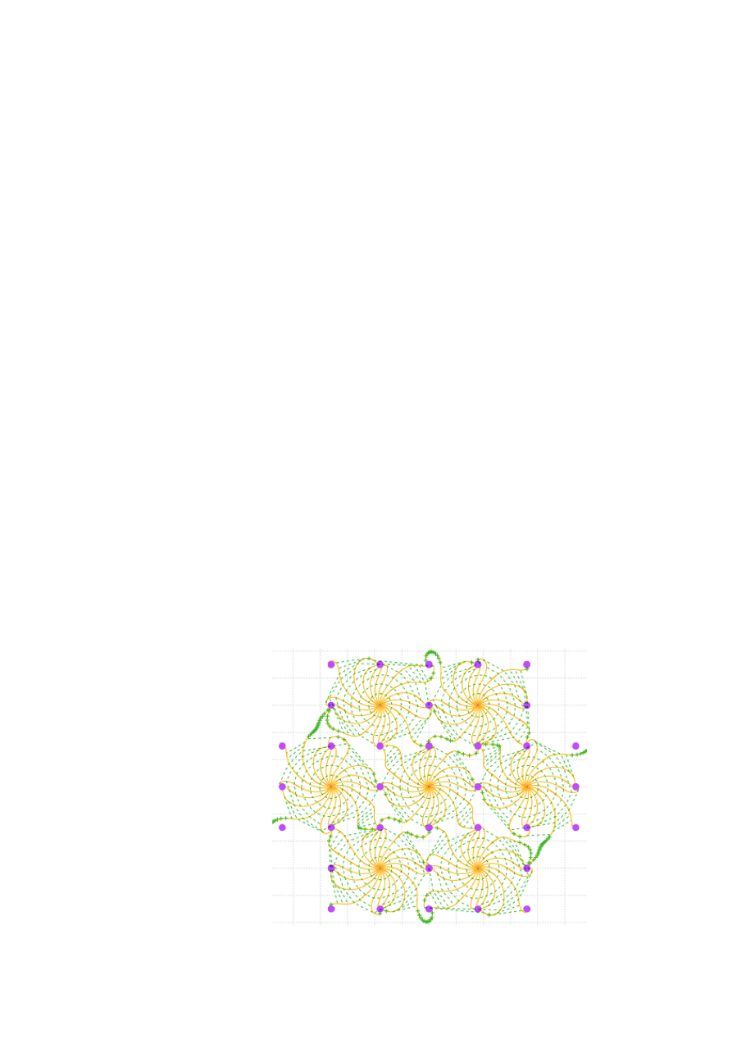
\includegraphics[width=0.5\linewidth]{figures/experimental_setup/electronsInCDC.pdf}
  \label{fig-sense-wires}
\end{SCfigure}


\begin{figure}
  \centering
  \includegraphics{figures/experimental_setup/axialLayers.pdf}
  
  \vspace*{1.5cm}
  
  \includegraphics{figures/experimental_setup/stereoLayers.pdf}
  \caption{Drawing sketching the axial (top) and stereo wires in the CDC. The skewing against the beamline of the stereo (bottom) wires is exaggerated. Taken from \cite{oliver}.}
  \label{fig-axial-stereo}
\end{figure}



\subsection{VXD}
 % DONE, Markus, Christian, Martin, Thomas H. -> fertig
  \chapter{Track Finder Theory and Multivariate Classification} \label{chapter-theory}

The track finders are implemented in the Belle~II analysis software framework for which a short introduction is given. More information can be found elsewhere~\cite{moll_basf2}. Afterwards a more detailed description of the theory of track finding and common figures of merit for all track finders are explained and discussed. As some parts of the track finders rely on the usage of multivariate classification the basic principle of boosted decision trees can be found in the end of the chapter.

\section{The Belle~II Analysis Software Framework (basf2)}

For simulation, data acquisition, data processing and analysis of the Belle~II experiment basf2 is used. Although -- going by its name -- it seems to be built on top of the old software framework used for the Belle experiment, it is a complete rewrite of the software using modern programming principles in the programming languages C++~\cite{cpp} and Python~\cite{python}. Together with external programming libraries e.g.\ ROOT~\cite{root} or EvtGen~\cite{evtgen} this framework builds the base for every software written for the experiment.

The software is divided into several packages -- each serving a distinct purpose or summarizing code for a single detector. Examples for the packages are CDC, SVD or tracking which is described in more detail in chapters~\ref{chapter-workflow}.

Each use of basf2 -- e.g.\ simulation, reconstruction or analysis -- consists of processing one or more so called \emph{paths} filled with \emph{modules}. These modules perform a dedicated small task e.g.\ simulating the $\PUpsilonFourS$-decay (the \texttt{EvtGen} module), writing out data to a root file (the module \texttt{RootOutput}) or performing a track reconstruction (for example with the module \texttt{TrackFinderCDCAutomaton}). The presence, the order, and the parameters of the modules are determined in \emph{steering files} written with Python. The modules itself can be written in C++ or Python. 

In these steering files a path is created, filled with modules and passed to the framework which handles loading the corresponding C++ libraries and calling the modules for every event that should be processed. An example of a small steering file for track finding can be found in listing~\ref{lis-steering-file}. Due to this extremely modular structure not only parallel processing but also debugging of intermediate steps can be performed much easily.

Because many modules need the data produced by other modules, there is a need for intermodular communication. This communication is performed within the framework with the help of a data store. It is used in the framework to store e.g.\ the hit information produced by the particles in the simulation or the found tracks after the track finding modules. The modules have read and write access to every \texttt{StoreArray} in the data store -- accessors to receive from and put objects on the data store. A visualization of the data flow between the modules created with the steering file in listing~\ref{lis-steering-file} can be found in figure~\ref{fig-viz-datastore}. The data store can be written to or read from disk using ROOTs own serialization mechanism together with data member dictionaries for the C++ classes created by the C++ interpreter of ROOT called CLING~\cite{cling}.

\begin{listing}
 \begin{lstlisting}[style=customP]
  # Import the needed basf2 package
  import basf2

  # Create a basf2 path
  path = basf2.create_path()

  # Add an input module to read from the file data.root
  path.add_module("RootInput", inputFileName="data.root")
  
  # Connect the gearbox, which is needed for loading the detector parameters
  path.add_module("Gearbox")

  # Add the Legendre track finder
  path.add_module("CDCLegendreTracking", WriteGFTrackCands=False)
  # Add the stereo Legendre finder
  path.add_module("StereoHitFinderCDCLegendreHistogramming",
                  SkipHitsPreparation=True,
                  TracksStoreObjNameIsInput=True,
                  WriteGFTrackCands=True)
  
  # Save the data store to a root file
  path.add_module("RootOutput")

  # Process the path
  basf2.process(path)

 \end{lstlisting}
 \caption[Python steering file to create a typical basf2 path.]{Python steering file to create a typical basf2 path. After loading the needed Python libraries the path is created and filled with the modules. In the end this path is processed and for each event the modules are executed in the given order and with their given parameters. For more information on the used modules see their documentation.}
 \label{lis-steering-file}
\end{listing}


\begin{figure}
 \centering
 \includegraphics[width=\linewidth]{figures/theory/dataflow.pdf}
 \caption[Visualization of intermodular communication.]{Visualization of the intermodular communication while processing the path implemented with the steering file described in listing~\ref{lis-steering-file}. The green boxes are entries in the data store. The ellipses are the processed modules. The red and blue arrows depict input and output to the modules. The dashed lines relations between the entries on the data store.}
 \label{fig-viz-datastore}
\end{figure}


\section{Working Principle of the CDC Track Finder in basf2}

One part of this thesis was the improvement and further development of the track finder modules for the CDC tracking detector. Therefore, the working principles of the two track finders for this detector are described here briefly. For more information on the Legendre track finder see~\cite{kronenbitter}. More information on the automaton track finder can be found in~\cite{oliver}.

The general purpose of a track finding algorithm is to partition all measured wire hits into exclusive sets of hits that originate from the same charged particle passing through the detector. It does so by making several assumptions on the charged particles producing the wire hits, e.g.\ the helical form of their trajectory and therefore the possible patterns of the hits. By fitting a mathematical model of a trajectory to these hits one gains information on the momentum and position of this particle. This part is called track fitting and is described in section~\ref{section-fitting}. The sets of hits possibly belonging to a charged particle are called tracks in the following.

The reason to have two track finders for the CDC is their different ansatz. The Legendre track finder is a so called global track finder whereas the automaton track finder is a local one. A global algorithm uses the information of all wire hits simultaneously. The Legendre track finder does this by applying a mathematical transformation to the wire positions which should in principle project all hits belonging to the same track onto the same coordinates. It is insensitive to missing hits but rather sensitive to high energy loss of the particles. A local algorithm however tries to use neighboring wire hits to construct clusters of hits. These clusters are then enlarged by using neighborhood relations again until a full track can be found. In opposite to a global track finding algorithm it can cope with energy loss and multiple scattering more easily. In the following these two principles are described in more detail.


\subsection{The Legendre Track Finder}
The principle of using the Legendre transformation for tracking algorithms in high energy physics experiments was first described by Alexopoulos~\cite{legendre}. It uses an extended version of the Hough transformation introduced by Paul V.C. Hough in 1962~\cite{hough}. The algorithm uses the fact that each trajectory in the $r$--$\phi$-plane of the detector can be described by a circle -- assuming no energy loss -- because of the direction of the applied magnetic field. In a first approximation one can also assume that each particle comes from the interaction point, which is valid for the bigger share of the decay products. Therefore the trajectory in the $r$--$\phi$ direction can be described by two parameters: the radius $R$ of the circle and the angle $\theta$ between an arbitrary, but fixed, axis and the tangent to the circle at the interaction point.\footnote{When dropping the last assumption (of tracks coming from the origin) one has to introduce another parameter -- often called $d_0$ -- which describes the minimal distance from the circle to the origin in the $r$-$\phi$ plane. It is easy to generalize the described algorithm to these three dimensions. In the moment this third dimension is however not implemented in the tracking software.}

Simplified, the idea is to calculate each trajectory that could have possibly created one of the axial hits and draw them all in a 2d histogram with the trajectory parameters $R$ (more precisely with $\rho = 1/R$) and $\theta$ as the coordinate axes. As there is only a small number of correct trajectories which are responsible for a great number of hits, there is a small parameter set which appears very often in the histogram. These parameters can then be used to create tracks.

For applying this algorithm, the $x$ and $y$ coordinate pair of every axial wire hit together with the drift length $d$ is transformed by the functions
\begin{align} x' = \frac{2x}{x^2 + y^2 - d^2}\ , \qquad y' = \frac{2y}{x^2 + y^2 - d^2}\ ,  \qquad d' = \frac{2R}{x^2 + y^2 - d^2}\quad \text{and} \label{eq-inverse} \end{align}
\begin{align}\rho(\theta) = x' \cos(\theta) + y' \sin(\theta) \pm d' \label{eq-legendre}\end{align}
into the Legendre space as shown in figure~\ref{fig-legendre-explained}. In the first step of the transformation, the wire hits are transformed to the inversed plane. With the transformation in equation~\ref{eq-inverse} each circular trajectory through the interaction point is mapped onto a line. The two trajectory parameters $R = 1/\rho$ and $\theta$ are now functions of the slope and the axis intercep of this line. After that, each drift circle is transformed into a pair of sinusoidal functions -- also called sinograms. This function $\rho(\theta)$ in equation~\ref{eq-legendre} is constructed in a way to use the fact that each trajectory of a charged particle responsible for a wire hit must touch the drift circle tangentially. Each point on the constructed sinusoidal functions corresponds to one possible trajectory of a particle which could have created such a hit. There are two sinusoidal functions because the osculation point can be on the far or near side of the drift circle -- the trajectory circle can circumscribe the drift circle or not. This is also shown in figure~\ref{fig-sinusodial}.

\begin{figure}
 \centering
 \includegraphics[scale=0.3]{figures/theory/legendre_1.png}
 \hspace*{1cm}
 \includegraphics[scale=0.3]{figures/theory/legendre_2.png}
 
 \vspace*{1cm}
 \includegraphics[scale=0.3]{figures/theory/legendre_3.png}
 \caption[Axial Legendre algorithm.]{Transformation of hits belonging to the same charged particle (upper left side) to the inversed plane (upper right side) and to the Legendre space with the characteristic sinusoidal functions (below). As described in the text, the circular trajectory is first transformed into lines and then into intersecting sinograms. Each sinogram includes all possible trajectory parameters which would have touched the hit from which the function was created. The intersection corresponds to the parameters of the trajectory and is marked with a red circle. For better visibility the wrong half of the sinograms is colored gray.}
 \label{fig-legendre-explained}
\end{figure}

\begin{figure}
  \centering
  \includegraphics[scale=0.27]{figures/theory/sinosodial_1.png}
  \hspace*{1cm}
  \includegraphics[scale=0.27]{figures/theory/sinosodial_2.png}
  \caption[Sinograms in the Legendre algorithm.]{The left picture shows one single oversized drift circle (black) and four trajectories (in color) that could have possibly created that hit as they touch the drift circle tangentially. The hit is transformed into two sinograms on the right picture. The drift circle lies on the outside of the green and red trajectories (gray sinogram = right side) and on the inside of the blue and yellow one (black sinogram = left side).}
  \label{fig-sinusodial}
\end{figure}


With using the information of a single hit one ends up with an infinite number of trajectory hypotheses. But as a charged particle passes many drift cells until it leaves the CDC detector -- in some cases up to 100 hits -- several wire hits are created with identical trajectory parameters. As these same parameters correspond to the same point in the Legendre space, the sinusoidal functions of the wire hits intersect in this point as can also be seen in figure~\ref{fig-legendre-explained}. The task of the Legendre algorithm now is to transform the hit coordinates and find those intersections.

Imperfections due to energy loss and material effects prevent the sinusoidal function from intersecting in one single point, but rather in a smeared area. To cope with this problem but still find intersections with a good performance a peak search in the binned Legendre space is applied. For each bin the number of sinusoidal functions passing this area is counted. The bin with the highest count is assumed to be the bin with the highest number of sinusoidal intersections. From the wire hits contributing to this bin a new track is created and the search is repeated with those hits deleted until a threshold in the bin entry is undercut. As the Legendre space is mostly empty, this procedure can be further improved in performance by refining the bin division from very coarse bin sizes to finer ones only for those bins which have a certain amount of sinusoidal functions in them. Because these bins are divided into 4 sub-bins with every refinement step the concept is called quad-tree search. The whole search is depicted in figure~\ref{fig-quad-tree-search}.

After finding possible hit subsets for the track candidates a post-processing procedure consisting of hit reassignment, hit deletion and track merging is applied to account for energy losses, trajectories not coming from the interaction point and finding inefficiencies.

\begin{figure}
  \centering
  \includegraphics[width=0.5\linewidth]{figures/theory/quad_tree.png}
  \caption[Quad tree search.]{Depiction of a quad tree search to find the bin with the most interceptions of sinograms shown in the smallest box in the center. Only the first round of the search without multicandidate search is shown for better visibility. Each color shows sinograms that belong to the same charged particle. Taken from~\cite{viktor_dpg}.}
  \label{fig-quad-tree-search}
\end{figure}


\subsubsection{Stereo Hit Finding}

In this thesis a refined algorithm for assigning stereo hits was implemented. The aforementioned Legendre track finding algorithm does only work for axial hits, as a precise position in $x$ and $y$ is needed for calculating the position in the Legendre space. Therefore it can not be applied for hits coming from stereo wires as they have a certain range of possible $x$--$y$-coordinates. But as soon as a trajectory is found using only axial hits, each stereo hit can be reconstructed to match the trajectory in such a way that its drift circle touches the trajectory circle of the candidate. As the stereo wire can be best approximated by a single line in 3d space the $z$ position is now also fixed. It is not possible to gain information on whether the drift circle is included in the trajectory circle or not -- for the same reason there were two sinograms. Therefore each stereo hit leads to two slightly different reconstructed $z$ positions. 

An ideal trajectory in the $s$-$z$ plane, with $s$ being the travel length in the circular two-dimensional projection, resembles a straight line analogous to the circle in the $r$--$\phi$ plane and can again be described by two parameters. This time these parameters are the slope\footnote{It is described by the angle $\lambda$ for consistency with the so called helix parameters, which are used for track parametrization.} $\tan \lambda$ and the distance $z_0$ on the $z$-axis to the interaction point. The plane spanned by these two parameters is analogous to the Legendre space in the axial case. As before each point corresponds to a certain trajectory. By using both reconstructed $z$ values from each stereo hit, two functions in this plane can be drawn which include every possible trajectory that would have passed the stereo hit. For axial hits these functions were given by the two sinograms. For stereo hits they are straight lines in the $\tan \lambda$--$z_0$-plane:
$$ z_0 = z_\text{rec} - \tan \lambda \cdot s_\text{rec} $$
with the reconstructed $z$ positions $z_\text{rec}$ and the reconstructed travel distance $s_\text{rec}$ which can be calculated using trigonometrical relations as the trajectory in a two-dimensional plane with fixed $z$ is approximated as a circle. The whole process can be seen in figure~\ref{fig-stereo-explained}. Again, a quad tree search is applied to search for the point with the highest number of interceptions which corresponds to the trajectory parameters compatible with the largest number of hits. This time only the single highest trajectory is stored as one single trajectory in the $r$--$\phi$ plane can only have one single trajectory in the $r$--$z$ plane. The whole algorithm is repeated for all other found axial-only trajectories. 

For most of the particles the energy loss has no influence on the $s$--$z$ motion because a momentum change would lead to the same deviations in the $z$ and the $s$ motion leaving $\tan \lambda$ approximately identical. Additionally, a non-zero distance to the interaction point is already accounted for, so post-processing is not needed here. See chapter~\ref{chapter-workflow} on the \texttt{SegmentTrackCombiner} for a description of how to cope with the remaining inefficiencies.


\begin{figure}
 \centering
 \includegraphics[scale=0.3]{figures/theory/stereo_1.png}
 \hspace*{1cm}
 \includegraphics[scale=0.3]{figures/theory/stereo_2.png}
 
 \vspace*{1cm}
 \includegraphics[scale=0.3]{figures/theory/stereo_3.png}
 \caption[Stereo Legendre algorithm.]{Stereo hit finding algorithm shown for a single track. The track trajectory in the $r$--$\phi$ (left upper) plane leads to two possible $z$ positions for each stereo hit (right upper). On the left upper side the trajectory together with the stereo wires projected to the $r$--$\phi$ plane is shown. In principle each stereo hit could have been created by an infinite number of tracks. Some of them are shown in green in the right upper picture. The dark green track is the correct hypothesis. Each line corresponds to a single point in the $\tan \lambda$--$z_0$-plane, which is shown below together with the correct trajectory parameters as a red diamond. The green diamonds correspond to the wrong light green lines in the right diagram. The $\tan \lambda$-$z_0$-lines for each hit as described in the text are also shown in black (correct hits) or in dashed (wrong hits).}
 \label{fig-stereo-explained}
\end{figure}


\subsection{The Automaton Track Finder}
Before doing the quad tree search the Legendre algorithm transforms each hit to the Legendre space in the same manner making it a global hit finder. The automaton track finder however is a local track finding algorithm using the neighborhood relations among the hits. It processes the hit information in two stages:
\begin{zlist}
  \item Clusterize the hits into groups (so called clusters) and create segments out of these clusters. A segment is a smaller part of a track limited by the superlayer bounds. 
  \item Use these superlayer segments and combine them into track candidates.
\end{zlist}

Both steps include the same problem: find the correct candidate among all combinations of items in a set. In the first step these items are the hit clusters, in the second step the segments. In both cases the problem is solved by applying a cellular automaton algorithm which is described briefly in the following. More information can for example be found in~\cite{cats},~\cite{kisel} and~\cite{oliver}. Each element in the set of items to be combined is modeled as a node in an acyclic directed graph. The edges in this graph represent the fact that a combination between adjacent elements is in principle possible. The implementation of this decision is of course dependent on the item type and the purpose of the cellular automaton. The typical problems in track finding software ensure that the graph is indeed cycleless and directed\footnote{It is directed because the natural flight direction of the tracks introduces a preferred direction and acyclic because the number of particles passing the same wire twice without leaving this superlayer is negligible.}. The cellular automaton now seeks to find the longest path in this directed graph, i.e.\ the path passing the highest number of nodes. To have more finer control on the output of the algorithm one can also apply weights to the edges and nodes of the graph. The output path is now not necessarily the longest path but the path with the highest sum of weights of the included edges and nodes. The cellular automaton algorithm finds this path by recursively traversing through the nodes and searching for the path with the highest sum of weights starting with this node. By passing this information to all parent nodes the output path can be easily found. The process is depicted in figure~\ref{fig-automaton}. If one is not only interested in the single best path, this procedure is repeated with the previously used items removed from the graph.

\begin{figure}
  \centering
  \begin{tikzpicture}[thick]
    \def\h{1}
    \def\x{2}
    
    \node[fill=kit-green50] (1) {1};
    
    \node[right=\x of 1] (dummy1) {};
    \node[fill=kit-green50, above=\h of dummy1] (2) {2};
    \node[fill=kit-green50, below=\h of dummy1] (3) {3};
    
    \node[fill=kit-green50, right=\x of dummy1] (4) {4};
    
    \node[right=\x of 4] (dummy2) {};
    \node[fill=kit-green50, above=\h of dummy2] (5) {5};
    \node[fill=kit-green50, below=\h of dummy2] (6) {6};
    
    \node[right=\x of dummy2] (dummy3) {};
    \node[fill=kit-green50, above=\h of dummy3] (7) {7};
    
    \draw[vecArrow, kit-orange50] (1) -- (2) node  [midway, sloped, above] {2.3};
    \draw[vecArrow] (1) -- (3) node  [midway, sloped, above] {1.7};
    \draw[vecArrow, kit-orange50] (2) -- (4) node  [midway, sloped, above] {0.6};
    \draw[vecArrow] (4) -- (5) node  [midway, sloped, above] {0.2};
    \draw[vecArrow, kit-orange50] (4) -- (6) node  [midway, sloped, above] {3.3};
    \draw[vecArrow] (5) -- (7) node  [midway, sloped, above] {0.1};
\end{tikzpicture}
\caption[Cellular automaton.]{Picture showing a typical acyclic directed automaton with nodes (green boxes) and edges (arrows) with their weights (number on the arrows). The algorithm outputs the orange path although the path 1-2-4-5-7 includes more nodes because its sum of weights is larger.}
\label{fig-automaton}
\end{figure}

The first step of the automaton track finder is to clusterize the hits into sets. A cluster of hits is defined as the largest set of directly adjacent hits in a single superlayer. This condition can also be weakened to allow for one-cell-wide gaps in the clusters. A typical event display with the found clusters is shown in figure~\ref{fig-clusters}. The segments which are built next are fully contained in one single cluster -- but one cluster can contain more than one segment when two tracks cross each other in this superlayer. To decide from which partition of hits in a cluster the segment should be built, the cellular algorithm is applied independently for each cluster. The nodes in the graph are given by the so-called facets. One facet is one of the possibilities of assembling three wire hits with those hits pairwise in close proximity to each other in two cases. Three possibilities for facets are shown in figure~\ref{fig-facets}. As can be seen in the figure, each wire hit already has a left-right passage information attached to it and combinations of the same three wires with different left-right information form different facets. With this left-right information a direction of flight can be defined (except for the sign). Configurable filters are used to trim down the created three-hit combinations to only compatible facets by limiting, for example, the angular deviation between the tangents to pairs of hits. Before applying the cellular automaton one also has to define the edges of the graph. Two facets have a directed connection in the graph if and only if the second and third hit of the first facet resemble the first and second hit of the second facet together with its left-right information and the angle between the defined directions of flight does not exceed a certain threshold. After performing the cellular automaton algorithm a set of paths including those facets is obtained. By collecting the hits included in those paths segments can be built.

\begin{figure}
  \centering
  \includegraphics[width=0.8\linewidth]{figures/theory/clusters.png} 
  \caption[Clusters in the automaton track finder.]{A typical event with colored clusters. The different colors have no particular meaning and are only for better distinction.}
  \label{fig-clusters}
\end{figure}

\begin{figure}
  \centering
  \includegraphics[width=\linewidth]{figures/theory/facets.pdf}
  \caption[Facets used in the automaton track finder.]{Three possibilities for facets with corresponding tangents (shown as red arrows) made from wire hits (in green). When changing the left-right hypothesis of one of the wire hits (which is not shown here) the facet is different than before. The sign of the direction vector can not be obtained with this local information. Taken from~\cite{oliver}.}
  \label{fig-facets}
\end{figure}

To construct the direction of flight and the tangents a distinct $x$-$y$ position for each hit is needed. For axial hits this position is given by the wire position but, stereo wires, in the absence of the $z$ position, do not have fixed coordinates in this plane. The problem can be solved by using the positions of the stereo wires for $z = 0$ in the cellular algorithm. This does not produce a large error as the reciprocal position of the stereo hits in one layer does not change much with different $z$ positions.

In this thesis different possibilities of combining the results of the Legendre track finder with the ones coming from the automaton track finder are investigated and implemented. For most of the cases the produced segments are used rather than full tracks for reasons described in later chapters. In order to run the local track finder as a standalone algorithm, the second step of creating track candidates out of the produced segments is also necessary. As this step is also performed using the cellular algorithm procedure the identities of nodes and edges have to be defined again. One natural choice would be to use the segments for the nodes and connect each pair of segments in the graph directly if their distance is small enough. Another approach is to use pairs or even three segments lying in consecutive superlayers. These groups of segments have at least one stereo segment in them giving the track piece $z$-information. This $z$-information can be used to create relations between those segment groups. Running the cellular automaton in a multipass manner leads to a collection of track candidates.


\section{The Used Figures of Merit}

For testing and developing and also for later usage in a physics analysis we need to compile numbers from the implemented track finding algorithms to see how well they work. There are three main classes of figures of merit to describe a track finding algorithm. All three classes listed here are described in more detail below. The three classes are:
\begin{itemize}
  \item the efficiency (e.g.\ the hit or finding efficiency, also for different particle types, momentum regions or areas in the detector)
  \item the error rate (e.g.\ the clone or fake rate)
  \item the computational performance (e.g.\ timing and memory consumption)
\end{itemize}

The last class should be quite clear and is measured by the basf2 measuring algorithms. As the tracking is part of the online reconstruction and may be at some point adopted for the high level trigger, the timing performance is very important. 

The other two classes can best be described by the algorithm that computes them. It starts with a full Monte Carlo (MC) simulation of generic $\PB\APB$ events with the full detector simulation afterwards. The created hits can then be grouped into distinct sets -- each describing a simulated track, called MC track candidate or MCTrackCand\footnote{They are also called track candidates to fit the naming convention of the track finder, although they are not candidates but rather correct tracks.}. Only those tracks that have at least 3 hits in the CDC are kept as a MCTrackCand -- otherwise they can not be fitted and even if there were a chance to find them via track finding, they could not be used for physics. After that, the simulated hits are used for track finding with the method to be evaluated. This can be done easily as the simulated hits are transformed into a format that is similar to the format that will be used later for the data coming from the experiment. After the track finder has produced a list of track candidates also, we can use the saved MC information to match tracks from the track finder to tracks from the MC algorithm by counting the number of hits they share. The different cases are depicted and described in table~\ref{tab-mc-track-finder}.

\begin{table}
  \centering
  \begin{tabular}{m{0.4\linewidth}m{0.5\linewidth}} \toprule
    \centering \includegraphics[width=0.8\linewidth]{figures/theory/fom_found.pdf} & There is a one-to-one connection between a MCTrackCand and a track from the track finder. The MCTrackCand is labeled found and the other track is labeled matched. \\ \midrule
    \centering 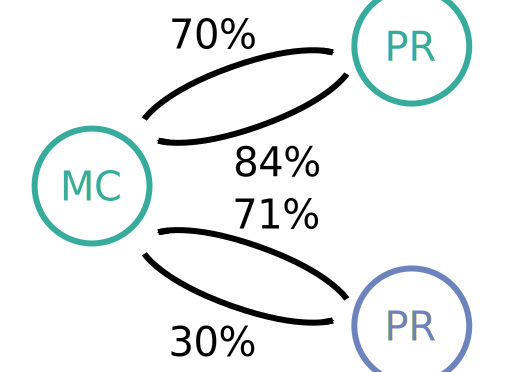
\includegraphics[width=0.8\linewidth]{figures/theory/fom_clone.pdf} & The MCTrackCand is found twice. The track from the track finder with the highest percentage (the green one in this example) is labeled matched, the other one is labeled cloned. The MCTrackCand is nevertheless labeled found. \\  \midrule
    \centering 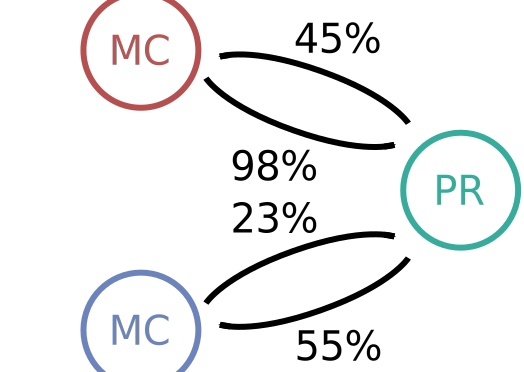
\includegraphics[width=0.8\linewidth]{figures/theory/fom_fake.pdf} & The track from the track finder is created with hits from many different MCTrackCands. As none of the corresponding hit ratios exceeds 66 \%, the PR track is called fake. There is no precise reason why the number 66\% was chosen. The hit ratios of the MCTrackCands itself do not play any role here. \\  \midrule
    \centering 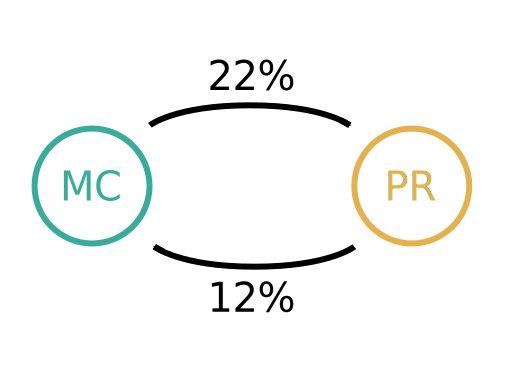
\includegraphics[width=0.8\linewidth]{figures/theory/fom_background.pdf} & The found track does not describe any of the MCTrackCands well (or well enough) -- but is made out of background hits. This track is also called a fake. \\ \bottomrule
  \end{tabular}
  \caption[Matching routine for compiling the FOM.]{This table shows the four different cases for the matching between MCTrackCands (MC, shown on the left side of the pictures) and tracks found by the pattern recognition algorithm (PR, on the right side). The different colors differentiate between different tracks. A connection between tracks shows that these two tracks share hits. The two percentages on the arrows are the percentages of hits they share in respect to the total number of hits in the MCTrackCand (arrows from MC to PR) or in the track candidate from the track finder (from PR to MC).}
  \label{tab-mc-track-finder}
\end{table}

The finding efficiency describes the rate of MCTrackCands which are labeled matched to the total amount of MC track candidates. Building this ratio can also be done for bins in various variables, e.g.\ perpendicular momentum ($p_T$), angle in the curling plane ($\phi$), number of tracks per event (multiplicity) and many more. A perfect track finder would have a finding efficiency of 100 \%. In most of the cases, the finding efficiency drops for tracks in a certain region of these variables -- e.g.\ low momentum tracks.
The hit efficiency is the mean of the ratios between the number of hits in the MCTrackCands matched to a non-fake track candidate to the number of hits in total of this track. A perfect track finder would have also a hit efficiency of 100 \%. In most of the cases the hit efficiency drops because of energy losses and deviations from the perfect trajectory form due to multiple scattering.
The fake and clone rates are the number of track candidates labeled as fake or clone by the matching algorithm divided by the number of found tracks in total. A perfect track finder would have both number set to 0 \%. A high fake rate is caused by a track finder with too loose cuts when putting together single pieces of tracks to a big track or by one which picks up background hits often. A track finder with a high clone rate on the other hand has too harsh cuts and often splits up tracks into more than one piece. To reduce statistical errors, these figures of merit are calculated for a high number of events.

\section{Track Fitting} \label{section-fitting}

Track finding algorithms have the task to partition the measured hits into sets with each set forming a track candidate. Afterwards the purpose of a track fitting algorithm is to fit a model for the trajectory to the measured information of the hits to gain the particles properties, e.g.\ the momentum or position. The model used for the fit can be very simple without taking into account material effects or energy loss. The track fitting algorithms implemented in genfit2~\cite{genfit} -- one of the external libraries used in basf2 -- however try to take care of the interaction of the particles with material by using the same algorithms in calculating these material effects that are used for simulating the detector geometry. As the calculation itself depends strongly on the track parameters this implies recalculating the material effects of the particle with every fitting step. Therefore an algorithm like the Kalman filter with its iterative approach is well-suited for track fitting.

The Kalman fitter algorithm~\cite{kalman} is based on the idea of iteratively adding measurements (e.g.\ the positions of the hits associated with this track) to the current state of the trajectory. Therefore the parameters change with every newly added hit and should in principle converge to the correct trajectory parameters. The change in the parameters is calculated by extrapolating a model of the trajectory with the current parameters to the plane of the next hit measurement and comparing this extrapolated position with the measured hit position. The deviation together with the errors of the measurement can be used to compile new parameters for the trajectory. By transversing back and forth several times through the whole hit set the final parameter estimation is found. One step in this procedure with only a small hit set is depicted in figure~\ref{fig-kalman}. As described before, the Kalman algorithm needs a current parameter state to calculate the extrapolation and the updated parameter set. As there is no possibility to gain a current parameter set before processing the first few hits the track finder must provide a starting seed for the track parameters.

\begin{figure}
 \centering
 \includegraphics[width=0.6\linewidth]{figures/theory/kalman.pdf}
 \caption[One step of the Kalman fitter procedure.]{Sketch of one step in the Kalman fitter procedure. The correct track parameters are depicted by the black trajectory. The green planes represent two sensors. The track passage positions -- the hit position measurements -- are shown as black circles. The current state of the fitting parameters is shown in gray. The state is extrapolated from the lower to the upper plane (gray dashed) and a new reconstructed position is calculated (gray circle on the upper plane). As there is a deviation between the current and the measured hit position, the current trajectory is changed according to the blue arrow.}
 \label{fig-kalman}
\end{figure}

When taking into account fake or background hits in a track, the Kalman fitter algorithm may not lead to good results anymore. As each hit is used for estimating the parameters of the trajectory a wrongly attached hit can give a wrong bias on these parameters. Therefore a weighting scheme is applied to all hits after each Kalman pass and this weight defines how strong a hit affects the final parameters. There are many different ways to do so, including elastic tracking and nonlinear filters~\cite{daf_fruh}. The one currently used for the tracking in the Belle~II software framework is the \emph{deterministic annealing filter} (DAF) introduced by Frühwirth and Strandlie. The procedure is as follows:
\begin{zlist}
  \item Set the weights of all hits to 1.
  \item Fit the track with a Kalman fitter taking into account the weights of each hit. \label{list-daf-loop-start}
  \item Recalculate the weight of each hit with the distance of the hit to the current trajectory hypothesis.
  \item Dismiss hits with a weight below a certain threshold.
  \item Continue with (\ref{list-daf-loop-start}) until a defined number of iterations is reached or the fit is converged.
\end{zlist}

To overcome the difficulties of badly chosen starting parameters of the fit that would lead to dismissing a large number of hits in the first iteration an annealing scheme is applied: each weight is transformed with a Maxwell-Boltzmann distribution depending on a ``temperature'' $T$ which is decreased with every iteration. In the first few iterations with a high temperature hits with a small weight are kept while in later iterations these hits are dismissed.

The fitting procedures are implemented in basf2 with the external library genfit2~\cite{genfit} -- a library for generic and experiment-independent track fitting. Only a small interface for accessing the genfit2 procedures from the basf2 code is implemented. See chapter~\ref{chapter-vxd} on the VXD momentum estimation for more information on this topic.

\section{Multivariate Classification}

During track finding -- especially in post-processing procedures -- many decisions must me made: whether a hit belongs to a track, whether two tracks should be merged, whether a track should be dismissed as fake, etc. In the context of inefficiencies and fakes due to background hits these decisions may depend on many input variables. Additionally there is the need to have a smooth transition between the two corner cases ``dismiss all'' and ``accept all'' to allow for subsequent optimization. This problem of deciding between two different possibilities for each input element (for example each track) is called a classification problem in statistics and there are many ways to deal with such problems (see for example references~\cite{cowan} or~\cite{blobel}). For most of the classification tasks in the track finding package for the CDC detector a classification algorithm known as \emph{boosted decision tree} (BDT) is used. In the following the main features are described. See reference~\cite{friedman} for more information on the algorithm and reference~\cite{keck} for details of the implementation.

The task of a classification algorithm is to decide whether an input element described by a feature vector $\vec x$ belongs to one class of elements or the other -- often these classes are called the signal and the background class. The classifier maps the multidimensional feature vector $\vec x$ to a one-dimensional output variable -- often between 0 and 1 -- which is designed in a way to separate signal and background by mapping signal like data to values near 1 and background like data to values near 0. The output can therefore be transformed to a probability for the input data to look like a signal sample and a configurable cut on the output can be used to distinguish between the two classes with a configurable purity or efficiency.

A decision tree is one possible implementation of such a classifier. It is created by dividing the parameter space of the feature vectors $\vec x$ into small hypercubes. As this is done by applying a division in one variable at the time a tree structure like in figure~\ref{fig-decision-tree} is formed. Each input data sample can then be mapped to the signal fraction of the hypercube it belongs to which is the output of of the tree for this element. This signal fraction is determined with a training sample of Monte Carlo generated events with known classification information. The cut values and variables are chosen in such a way as to maximize a separation measure, e.g.\ the gini impurity that models the gain introduced this separation. The measure is also calculated using the training sample.

Because the chosen cuts depend strongly on the training sample a single decision tree can easily be overtrained. A classifier is called overtrained when its separation power on the testing data set is much better than on an independent testing sample because instead of generalizing the training data it fits its output function to the training data perfectly well. An overtrained classifier can not anything else than those cases that were present in the training set. To avoid overtraining an algorithm known as boosting is applied to the decision tree. This algorithm creates a whole set of decision trees iteratively. Each decision tree is trained to separate the items classified wrongly by the one before. It does so by applying weights to the items. The final output of the classifier is a weighted sum of all single trees. By limiting the depth of a single decision tree it avoids overtraining but because of the huge number of trees it still has a great separation power.

\begin{figure}
  \centering
  \begin{tikzpicture}[thick]
    \node[module] (alldata) {Decision Tree};
    \def\h{1}
    \def\x{0.8}
    \node[module, text width=6em, fill=kit-orange50, below=0.25 of alldata] (cut1) {$x_3 > a$?};
    \node[below=\h of cut1] (dummy1) {};
    \node[below=\h of dummy1] (dummy2) {};
    \node[below=\h of dummy2] (dummy3) {};
    \node[module, text width=6em, fill=kit-orange50, left=3*\x of dummy1] (cut2a) {$x_1 > b$?};
    \node[module, text width=6em,fill=kit-orange50, left=\x of dummy2] (cut3a) {$x_7 > d$?};
    \node[module, text width=6em,fill=kit-orange50, left=5*\x of dummy2] (cut3b) {$x_5 > e$?};
    \node[module, text width=6em,fill=kit-orange50, right=3*\x of dummy1] (cut2b) {$x_2 > f$?};
    \node[module, text width=6em,fill=kit-orange50, right=\x of dummy2] (cut3c) {$x_4 > g$?};
    \node[module, text width=6em,fill=kit-orange50, right=5*\x of dummy2] (cut3d) {$x_6 > h$?};
    
    \node[module, text width=6em, left=\x of dummy3] (result3a) {10 signal events};
    \node[module, text width=6em, left=5*\x of dummy3] (result3b) {328 signal events};
    \node[module, text width=6em, right=\x of dummy3] (result3c) {4136 signal events};
    \node[module, text width=6em, right=5*\x of dummy3] (result3d) {4 signal events};
    
    
   \draw[vecArrow] (cut1) -- (cut2a.north);
   \draw[vecArrow] (cut1) -- (cut2b.north);
   \draw[vecArrow] (cut2a) -- (cut3a.north);
   \draw[vecArrow] (cut2a) -- (cut3b.north);
   \draw[vecArrow] (cut2b) -- (cut3c.north);
   \draw[vecArrow] (cut2b) -- (cut3d.north);
\end{tikzpicture}
\caption[Decision Tree.]{A decision tree dividing a 7-dimensional parameter space into 4 hypercubes with seven cuts in three layers. The last layer is used to generate the output of the decision tree by counting the number of signal events in this hypercube in the training sample.}
\label{fig-decision-tree}
\end{figure}


 % DONE, Markus, Christian, Martin, Thomas H. -> fertig
  \chapter{Track Finding in basf2} \label{chapter-workflow}

After having described the principle of the track finders implemented in basf2 in the previous chapters, the actual changes to the software implementation during this thesis is discussed in this chapter. Before going into detail, the figures of merit of the two track finders showing their advantages and drawbacks are presented in the first section. After a short introduction in the general structure, the newly implemented background hit finder and the performed improvements on the stereo Legendre track finder are shown. Then the newly written \texttt{SegmentTrackCombinerModule} is described. The chapter ends with a section on general tools how to improve the found track candidates and an outlook.

\section{FOM of the two track finders}

Standalone legendre + standalone local
Legendre (old!): Finding efficiency, d0 influence, purity
Local: Segment purity, Finding efficiency; Clone + Fake-Rate of both track finder (Local with combined Segments)
Timing.

\todo{pictures: Finding efficiency legendre over pt, d0 influence, purity as histogramm}
\todo{pictures: Timing of legendre + stereo and local}
\todo{pictures: Purity of segments as hist, Finding efficiency over pt + d0}

\section{The \texttt{TrackFindingCDC} Package}
As presented in the section before, the two track finding algorithms have different characteristics. To use the benefits of both, a combined approach is suited best. The proposed workflow as a result of the analysis done in this thesis is presented simplified in figure~\ref{fig-workflow}. The idea is to run both track finders on the same (full) set of hits and combine the resulting tracks/segments afterwards. Another solution is to use only the hits that are not already used by the first track finder in the second one. This proposed approach has an increased computing time in contrast to this solution but has some other advantages: 
\begin{itemize}
 \item If a track is found by both track finders, the probability of it being a fake is very small.
 \item If a track is only found partly by the first track finder, the second algorithm will probably not find the rest as only some hits are unused. When both track finders use the full set of hits, the combined tracks include most of the hits of a track.
 \item Both track finder can be optimized independently. It is even possible to run only one of them to save computing time or for special detector setups (e.g. for cosmic runs) without changing much in the software configuration.
\end{itemize}

\begin{figure}
  \centering
  \begin{tikzpicture}[thick]
    \node[module] (simulation) {Simulation or Experiment};
    \node[module, below=1 of simulation] (background) {Filter Background Hits};
    \draw[vecArrow] (simulation) -- (background) node [midway, anchor=west] {CDC Hits};
    \node[module, below right=1.8 of background] (local) {Local Track Finder};  
    \node[module, below left=1.8 of background] (global) {Global Track Finder};  
    \draw[vecArrow] (background) -- (local) node [midway, auto=false, anchor=south, sloped] {CDC Hits};
    \draw[vecArrow] (background) -- (global) node [midway, auto=false, anchor=south, sloped] {CDC Hits};
    \node[module, below right=1.8 of global] (combiner) {Segment and Track Combiner};  
    \draw[vecArrow] (local) -- (combiner) node [midway, auto=false, anchor=south, sloped] {Segments};
    \draw[vecArrow] (global) -- (combiner) node [midway, auto=false, anchor=south, sloped] {Tracks};
    \node[module, below=1 of combiner] (fitter) {Track Fitter};
    \draw[vecArrow] (combiner) -- (fitter) node [midway, auto=false, anchor=west] {Tracks};
  \end{tikzpicture} 
 \caption[Proposed workflow in the CDC tracking]{The proposed workflow and combination of the two track finders in the CDC detector. The green boxes refer to one or a few modules. The arrows describe parts of the data flow between the modules. For clarity not all necessary parts are shown here.}
 \label{fig-workflow}
\end{figure}

For better interconnectivity between the track finders, they share a large code basis including common data objects and module system in addition to the already given framework by basf2. Combining the code basis of the two track finders was also part of this thesis. The common software design consists e.g.\ of a common singleton (called \texttt{CDCWireHitTopology}) saved in the data store which is responsible for storing the used-flag of the CDC hits and their connection to other objects (like clusters or segments). Also the in- and output of all tracking modules in the CDC is handled by shared code which makes changes in the data flow much easier.

Figure~\ref{fig-workflow2} shows the same workflow as presented im figure~\ref{fig-workflow} (except the simulation and the track fit), but now with the correct module names and the relevant data flow. The \texttt{CDCWireHitTopology} singleton is not parts of the modules but gets used by all modules to check the usage flag and the geometrical information of the wire hits. The modules in the path are described in the following in more detail.

\begin{description}
  \item[Wire\-Hit\-Topology\-Preparer] This module receives the simulated or measured hit information from the CDC detector and connects it with the geometrical information from a database. All hits with configurable flags are saved in the wire hit topology object which is stored as a persistent \texttt{StoreObj} in the data store.
  \item[Segment\-Finder\-CDC\-Facet\-Automaton\-Dev] The module is the first part of the local track finder as described in chapter~\ref{chapter-theory}. As the clusterizer is one part in the cellular automaton used in this algorithm it is -- apart from creating segments -- also used for separating signal and background hits. This filter is described in section~\ref{section-background}. The rest of the module was not developed in this thesis and can be found elsewhere~\cite{oliver}. As all CDC tracking modules communicate over the wire hit topology object, the background flag is propagated to all other modules.
  \item[CDC\-Legendre\-Tracking] Running the axial Legendre track finder with the quad tree search is done in this part as described also in chapter~\ref{chapter}. It uses the full wire hit set (except the background hits). It has also some post-processing steps included directly after the search, which were analyzed and improved in this thesis. \todo{describe?}
  \item[Track\-Quality\-Asserter\-CDC] Although all track finding algorithms are highly optimized there is a need for quality improvement tools for the resulting track candidates. To make this step configurable for later adjustment and to share the code basis between the algorithms, tools for track corrections were developed in this thesis (see section~\ref{section-quality}). They can be used in the modules directly or via this module which is used in two positions in the path with different configurations.
  \item[Stereo\-Hit\-Finder\-CDC\-Legendre\-Histogramming] After the axial track finder created tracks, the get used in this module to add stereo hits with a quad tree search also. This module was rewritten from scratch in this thesis and is described in section~\ref{section-stereo}.
  \item[Segment\-Track\-Combiner\-Dev] The final step (except for quality improvements) is the combination of the results of the global and local track finder which is handled by this module. It was also created in this thesis and is presented in section~\ref{section-combiner}.
\end{description}

\begin{figure}
  \centering
  \begin{tikzpicture}[thick]
    \node[module, text width=12em] (hits) {{Wire\-Hit\-Topology\-Preparer}};
    \node[module, below=1 of hits, text width=12em] (segment) {{Segment\-Finder\-CDC\-Facet\-Automaton\-Dev}};
    \node[module, below=1 of segment, text width=12em] (axial) {{CDC\-Legendre\-Tracking}};
    \node[module, below=1 of axial, text width=12em] (quality1) {{Track\-Quality\-Asserter\-CDC}};
    \node[module, below=1 of quality1, text width=12em] (stereo) {{Stereo\-Hit\-Finder\-CDC\-Legendre\-Histogramming}};
    \node[module, below=1 of stereo, text width=12em] (combiner) {{Segment\-Track\-Combiner\-Dev}};
    \node[module, below=1 of combiner, text width=12em] (quality2) {{Track\-Quality\-Asserter\-CDC}};
    
    \node[cloud, right=3 of hits] (topo) {{CDCWireHitTopology}};
    
    \draw[vecArrow] (hits) -- (topo) node [midway, anchor=south, sloped, auto=false] {All CDC Hits};
    \draw[vecArrow] (topo) -- (segment) node [midway, anchor=south, sloped, auto=false] {All CDC Hits};
    \draw[vecArrow] (segment.east) -- (topo.south) node [midway, anchor=north, sloped, auto=false] {Filtered CDC Hits};
    \draw[vecArrow] (topo.south) -- (axial.east) node [midway, anchor=north, sloped, auto=false] {Filtered CDC Hits};
    \draw[vecArrow] (axial) -- (quality1) node [midway, anchor=west] {Axial Tracks};
    \draw[vecArrow] (quality1) -- (stereo) node [midway, anchor=west] {Corrected Axial Tracks};
    \draw[vecArrow] (stereo) -- (combiner) node [midway, anchor=west] {Full Tracks};
    \draw[vecArrow] (combiner) -- (quality2) node [midway, anchor=west] {Combined Tracks};
    \draw[vecArrow] (segment.west) to[out=-150, in=150] node [midway, anchor=east] {Segments} (combiner.west) ;
  \end{tikzpicture} 
 \caption[Detailed workflow in the CDC tracking]{The detailed workflow for the track finding procedure for the CDC detector with the correct names of the modules as in the software. The green boxes refer to one modules. The red ellipse is an object on the data store. Some dependencies between the modules are shown as arrows.}
 \label{fig-workflow2}
\end{figure}

\section{The Background Hit Finder} \label{section-background}
The beforementioned track finders are tuned to not pick up background hits into a found track candidate or even form a candidate from background hits only. Nevertheless even a single background hit per track can lead to a reduced momentum resolution or can even cause the fit to fail completely. Together with the reduced combinatorics and therefore reduced computing time when throwing away unusable hits there is the need to distinguish between signal and background hits even before the tracking starts. This is the purpose of the background hit finder module described in this section.

For deciding if a hit is to be used in the track finder, the module uses implemented filters. As these filters are used widely in the whole CDC tracking framework, they will be described here in more detail. To filter out bad hits, not only the information of one hit but the information of the clusters constructed in the local track finder is used. As described in chapter~\ref{chapter-theory} they are created by clusterizing all CDC hits in such a way that one cluster includes the maximum number of connected hits. Two hits are called connected if there is no non-fired wire geometrically between them. Because of the modular framework and the reusable \texttt{CDCWireHitTopology} it is possible to run the local track finder with the clusterizer before the legendre track finder and propagate the background information to the following tracking algorithms. 

Figure~\ref{fig-clusters} in chapter~\ref{chapter-theory} shows an event display in the $r$-$\phi$-plane with the clusters drawn in different colors. Figure~\ref{fig-cluster-hit-purity} shows the hit purity of ANZAHL of the clusters from typical events. The hit purity is computed as the ratio between the number of hits in a cluster which belong to a signal track divided by the number of all hits (including the ones coming from background only). As can be seen clearly in this histogramm a cluster is either full of background or full of signal hits - for that throwing away a background cluster does not involve deleting hits that are needed for signal tracks.

\begin{figure}
  \todo{figure}
  \caption{}
  \label{fig-cluster-hit-purity}
\end{figure}


In every event, each formed cluster is passed to the chosen filter with the chosen filter parameters. This filter can return every number as a result including the C++ std::nan, which is used as the value for indicating that the cluster should not be used further for track finding as it is marked as background by the filter. Actually, the non NaN numbers returned by the filter are not used further in the following algorithms and are just described here for later reference. 

This filter algorithm is a very general one and leaves the possibility open to compare many different filters. For this as well as for any other used filter in the CDC tracking, five filters are implemented by default which can be switched by using module parameters. These filters are:

\begin{description}
  \item[BaseFilter] is a filter that neglects every item - it is just for basing every other filter on a common ground class and not for usage.
  \item[AllFilter] is the counterpart of the BaseFilter and accepts all items. It can be used for testing purposes to make a filter fully transparent.
  \item[SimpleFilter] is a filter based on self-implemented cuts. The variables to cut depend on the planned usage of the filter and need to be implemented by the programmer.
  \item[TMVAFilter] is based on a trained boosted decision tree. It passed the variables defined in a so called VarSet to the BDT and returns the result to result between 0 and 1. If the result is lower than a certain cut definable on runtime, the TMVAFilter returns std::nan. The variables and their calculation can be freely defined by the programmer. In most of the cases the performance of a well-trained TMVAFilter exceeds the one of a simple filter.
  \item[RecordingFilter] returns a constant defineable on runtime and can therefore not directly be called a filter. Instead its purpose is to write the same variables as the TMVAFilter uses together with a truth information of every incming item into a ROOT TNTuple. The output file with this TNTuple can later be used to train the BDT to categorize according to the truth information. This filter can of course only be used on simulated data.
  \item[MCFilter] filters the items according to the truth information compiled with the MC information that also the recording filter uses. 
\end{description}

As an example for the mentioned VarSet, the variables for distinguishing the background clusters from the signal clusters is described in table~\ref{tab-varset-cluster}. The truth information used for the BDT training is also described there. The trained BDT has PARAMETERS... EVENTS were used for training. 

\begin{table}
  \todo{var set}
  \caption{}
  \label{tab-varset-cluster}
\end{table}


After the training procedure the corresponding TMVAFilter can be used. The results are summerized in figure~\ref{fig-result-background-hit-finder}. 

\begin{figure}
  \todo{ROC curve}
  \caption{}
  \label{fig-result-background-hit-finder}
\end{figure}


\todo{Results for Clusters/Hits, Results for Legendre Finder}

\todo{describe axial or not?}
% \section{Improvements on the Axial Legendre Track Finder}
% Is already very good and advanced. 

% \subsection{The class \texttt{QuadTreeProcessorTemplate}}
% \subsection{Postprocessing after the track finding}
% \subsection{Results}
% Timing

\section{Improvements on the Stereo Legendre Hit Finder} \label{section-stereo}
\subsection{Implemented algorithm}
\subsection{Results}
Timing

\section{The \texttt{SegmentTrackCombinerModule}} \label{section-combiner}
\subsection{Principle of the Segment Track Combiner}
+ Task
\subsection{Used Filters}
\subsection{Results}

\section{The \texttt{TrackQualityAsserterCDCModule} and the \texttt{TrackQualityTools}}  \label{section-quality}

Fitting problem. Implemented quality tools (description). Some event displays.

\section{Further Approaches}
\subsection{Quad tree search with segments}
Benefits: Purity high, more or less no reassignment needed. RL-information already present, lower combinatorics = more then one axis possible?

More than one possibility to do that: axial + stereo or only stereo or only axial, when should a segment belong to this legendre bin?

\subsection{VXD-CDC-Merger before fitting}
Benefits: Possible better efficiency (no loss because of fit). Faster, less fakes, better finding efficiency (because a track is kept which would be maybe deleted by a quality tool)

Ho to do it: BDT with trained variables. First results. % DONE, Martin -> fertig
  \newcommand{\dedx}{$\mathrm d E / \mathrm d x$ }
\chapter{Momentum estimation of slow pions with the ADC in the VXD}

When looking onto the typical momentum distribution of the particles flying through the tracking detectors as show in figure \ref{fig-particles-momentum} it is clear that there is a significant amount of so called slow pions with momenta in the order of $\unit[100]{MeV}$. These particles get produced more or less at the interaction point and because of their small momentum and therefore high curvature and their huge energy losses they can not be detected in the CDC tracking detector. This means they can only be measured in the VXD. Because of the small radius of the VXD and the resulting small number of independent measurement points, the momentum resolution is very poor as it can be seen in the Glückstern formula
\begin{align*}
 \frac{\sigma_{p_T}}{p_T} = \sqrt{\frac{720}{N + 4}} \sigma_x \frac{p_T \text{[GeV]}}{0.3 q B \text{[T]} L^2}
\end{align*}
where L is the length of the track in the detector and $N$ is the number of measurement points. Decreasing the magnetic field would decrease the curvature of the low momentum pions and would therefore make them detectable in the CDC also increasing the number of measurement points. But this would also make the resolution of the high momentum particles very poor. In this thesis a different approach is chosen. Together with the measured positions for each found VXD sensor hit an independent momentum estimation based on the energy loss per length of the particles in this sensor is calculated and used in the trajectory fit after the track finding. These added measurements bias the fit towards the correct momentum and can therefore help to increase the momentum resolution.

\begin{figure}
 \centering
 \includegraphics[width=0.8\linewidth]{figures/vxd/momentumDistribution.png}
 \caption{Momentum distribution split by different particle types as generated by the simulation. As this simulation is modeled after the physical branching fractions the here shown distribution is also the expected observation in the experiment.}
 \label{fig-particles-momentum}
\end{figure}

As it was shown in previous studies \cite{robert}, the momentum resolution compared to the result of the helix fit with the positions only can be increased by using the information from the energy loss of all hits in the track together. In the quoted paper an advanced summation was used to build a mean energy loss of the slow pions which was transformed to a momentum by a predetermined formula. This momentum estimation was then compared to the one coming from the helix fit. To increase the resolution even more the two different approaches are combined in the presented algorithm.

In figure \ref{fig-dedx-over-p} the energy loss per travel length in the VXD sensors for low momentum pions is shown. How these numbers are calculated is described in the next sections. As it can be seen the \dedx increases with falling momentum of the particles. This relation can be also seen in the already quoted Bethe formula \ref{form-bethe} in chapter \ref{chapter-ex} which can be reduced to 
\begin{align}
 -\left \langle \dd{E}{x} \right\rangle \approx \frac{4 \pi n z^2}{m_e v^2} \left( \frac{e^2}{4 \pi \varepsilon_0} \right)^2 \ln \left( \frac{2 m_e v^2}{I} \right) \label{form-bethe-simpl}
\end{align}
for small particle energies. The equation can be used to calculate the momentum using the energy loss per travel length. But as this formula describes the averaged energy loss it is only correct for a small number of cases. The variance in the energy loss is distributed according to a landau distribution which is described later in more detail. This deviation from the Bethe formula decreases the momentum resolution of the estimation based on the energy loss.

\begin{figure}
 \centering
 \includegraphics[width=0.8\linewidth]{figures/vxd/dedx.png}
 \caption{\dedx information of the VXD clusters of approximately 100000 pions in the momentum range from 50 to 120 MeV. The averaged energy loss can be described by the Bethe formula. The distribution of energy losses for a given momentum is distributed according to a landau distribution which is described later in more detail. To transform the \dedx value to a momentum the red estimator curve is used later.}
 \label{fig-dedx-over-p}
\end{figure}


\section{Prestudies on the distribution of dE/dX in the VXD}

For the following studies an event sample of slow pions in the momentum range between $\unit[50]{MeV}$ and $\unit[120]{MeV}$ is used. It is simulated using the particle gun with 10 particles per event evenly distributed among the momentum range and between the two charge modes. The sample is split into different event samples for testing and fitting. The standalone VXD track finder or the MC track finder for reference is used to create tracks out of the simulated VXD hits. As the finding efficiency of the standalone VXD track finder depends heavily on the momenta of the particles, the distribution of the found tracks is not flat any more as it can be seen in figure \ref{fig-vxd-finding-efficiency}. A typical event display can be seen in picture \ref{fig-vxd-event-display}.

\begin{figure}
 \centering
 \includegraphics[width=0.48\linewidth]{figures/vxd/finding_efficiency.png}
 \includegraphics[width=0.48\linewidth]{figures/vxd/finding_efficiency.png}
 \todo{correct picture}
 \caption{Momentum distribution of the simulated pions as found by the VXD track finder (left) and the MC track finder (which has the simulated truth information, right). The finding efficiency decreases with lower momenta as the number of hits in the VXD is lower for slow pions and the energy loss is stronger. The MC track finder has also not a flat distribution of momenta as it only uses those particles for tracks which have at least 3 hits in the VXD detector.}
 \label{fig-vxd-finding-efficiency}
\end{figure}

\begin{figure}
 \centering
 \includegraphics[width=0.8\linewidth]{figures/vxd/event_display.png}
 \caption{Typical event display of one event used for analyzing the momentum estimation for the fitting procedure in the helix fit. The blue box depicts the inner wall of the CDC. As it can be seen, most of the particles do not reach into the drift chamber and can only be detected with the VXD sensors.}
 \label{fig-vxd-event-display}
\end{figure}

Before calculating the function to transform the \dedx value to a momentum estimation and using this information in the helix fit some prestudies are performed to check for the consistency of the input data. They are shown here for reference too.

For calculating the path length used in \dedx the correct position of the hit and the sensor information is needed. This information is provided by the clusters used in the track finder. Its results can be seen in figure \ref{fig-cluster-position} where the distance to the beam pipe over the z position is shown for some SVD hits. This position is later used to calculate the path length of the tracks in the sensor region.

\begin{figure}
 \centering
 \includegraphics[width=0.8\linewidth]{figures/vxd/cluster_positions.png}
 \caption{Picture showing the simulated hit information of the first 1000 clusters in the event sample. The color code separates between the sensor ID property of the clusters.}
 \label{fig-cluster-position}
\end{figure}

Instead of using the deposited charge in every sensor directly the ADC count value of every sensor is used. This ADC count comes directly from the digitalization process and does therefore not rely on any calibration process. As it is directly proportional to the deposited energy and the parameters of the transformation function from \dedx to the momentum have to be determined by a fit in either way, the ADC count is used as a measure for the energy deposition. Picture \ref{fig-adc-count} shows the the \dedx value calculated with this ADC count for the two different detectors SVD and PXD. As it can be seen, the calibration coefficients to the correct deposited energy are different for the two detectors and therefore the two distributions are not superimposable. To cope with this fact the ADC counts coming from the PXD sensors get multiplied by a factor of 0.565868 which was calculated on data. The resulting distribution is shown in the right subplot of figure \ref{fig-adc-count}. This calibration is mainly done to be able to treat both hit types in the same manner later. 

\begin{figure}
  \centering
 \includegraphics[width=0.48\linewidth]{figures/vxd/dEdXUncalibrated.png}
 \includegraphics[width=0.48\linewidth]{figures/vxd/dEdXCalibrated.png}
 \caption{Distributions of the uncalibrated (left) and the calibrated (right) ADC counts of the PXD and SVD hits. Only clusters found by the VXD track finder are shown here.}
 \label{fig-adc-count}
\end{figure}

\subsection{Calculation of the path length in the clusters}
The \dedx value in every cluster can be calculated using the calibrated charge as described above and the length of the path the particle travels in the sensor region. There are five ways to calculate this path length. All of them are implemented in the code basis.
\begin{zlist}
 \item Using the correct (simulated) MC trajectory information of the tracks at the position of the clusters, \label{list-mc}
 \item Using the current trajectory parameters while fitting,
 \item Using the related MC trajectory at the origin,
 \item Using the trajectory parameters estimated by the track finder without MC truth information,
 \item Using the thickness of the cluster.
\end{zlist}

The different possibilities are ordered by their anticipated correctness. The two MC modes are only implemented for reference as they can obviously not be used in the later detector measurement. How the current trajectory parameters are deduced in the fit is described later.

Besides the last possibilities all modes rely on calculating the path length of a trajectory using their helix parameters. As the calculated path lengths are very small, this is done without taking into account energy loss or material effects. The procedure is as follows:
\begin{zlist}
 \item Take the position of the cluster hit (the point where the trajectory enters the VXD sensor) and calculate the distance to the beam line. This is called the inner radius of the cluster.
 \item Add the sensor thickness to this radius to gain an estimation of the outer radius of the sensor.
 \item Calculate the arc length between these two radii and from this arc length the distance between the two penetration points of the helix through the sensor using trigonometrical relations.
\end{zlist}

This procedure is correct for most of the time but fails in some rare cases. Some examples are shown in figure \ref{fig-errors-in-path-length}. As it can be seen in the pictures, errors in the calculation occur mainly for particles which have their apogee\footnote{The apogee is the opposite to the perigee - the point on the helical trajectory the most far away from the interaction point} in the sensors. As the VXD sensors have only a very thin thickness the probability for such particles is very rare. Therefore these cases do not bias the momentum measurement much. Also as the calculation error can only occur in the most outer sensor touched by the particles all other sensors give correct momentum estimations. A short preliminary study shows that only about 0.4 \% of the particles are affected.

\begin{figure}
  \centering
  \raisebox{-0.5\height}{\includegraphics[scale=0.3]{figures/vxd/pathlength1.pdf}}
  \hspace*{1.5cm}
  \raisebox{-0.65\height}{\includegraphics[scale=0.3]{figures/vxd/pathlength3.pdf}}
  \hspace*{0.5cm}
  \raisebox{-0.5\height}{\includegraphics[scale=0.3]{figures/vxd/pathlength4b.pdf}}
  \caption{Exemplary cases of path length calculations. The algorithm fails in the second and last case. In the second case it returns the width or the length of the sensor instead. In the last case it wrongly adds the orange part of the path length to the correct one. Because of the geometrical dimensions of the sensors these two cases are very rare.}
  \label{fig-errors-in-path-length}
\end{figure}

In figure \ref{fig-pathlengths} the distribution of the path lengths from the simulated MC truth values is shown. As most of the particles go more or less straight through the sensors, there are two peaks in the distribution - one for each hit type as the two types PXD and SVD have a different thickness. Deviations from the thickness come from curling particles. The fact that there are only few tracks with very high deviations from the thickness values verifies th claim that the helix calculation is wrong only for very rare cases.

The second subplot shows the distribution of the residuals of the other four path length calculations to these reference values as a violin plot.

\todo{Beschreibung!}

\begin{figure}
 \centering
  \includegraphics[width=0.7\linewidth]{figures/vxd/pathLengths.png}
 \caption{The plot shows the path length distribution for the two sensor types as a result of the simulation. This distribution is used for reference in the right plot which shows the residuum distribution of the other path length calculation modes.}
 \label{fig-pathlengths}
\end{figure}

\subsection{Transformation function from dE/dX to momentum}

For calculating a momentum estimation from the \dedx value the inverted function of equation \ref{form-bethe-simpl} is needed which can not be calculated analytically. Therefore a much easier model function
\begin{align}
 p(\mathrm{d}E/\mathrm{d} x) = \frac{a}{(\mathrm{d}E/\mathrm{d} x - b)^2} + c \cdot \mathrm{d}E/\mathrm{d} x + d \label{form-model}
\end{align}
with the free parameters $a, b, c$ and $d$ is fitted to the \dedx-momentum-values where \dedx is calculated with path lengths from mode (\ref{list-mc}) and the momentum is taken from the MC simulation at this cluster (so including energy loss by material effects).

The fitting parameters can not be determined by fitting the model function to the whole distribution at once as shown for example in figure \ref{fig-dedx-over-p}. The reason is that because of the landau distributed energy loss the number of outliers is too high and caused the fit to fail. An example of the landau distribution showing the large amount of outliers deviating from the mean energy loss is shown in picture \ref{fig-landau}. This is why a reduce approach is chosen here: First the \dedx-range is split into several small bins. In each of them the momentum distribution is build. This distribution is then fitted with a landau or a normal distribution. Mathematically, the momentum distribution in these \dedx-bins is neither distributed according to a landau nor a normal distribution but the correct form can not be calculated analytically and these two distributions describe the data best.\footnote{The correct form of the distribution can be calculated by integrating over parts of the landau distribution folded with the inverted Bethe-equation, which is not analytically solvable.} The resulting parameters of the distributions (the mean of the gauß or the location parameter of the landau distribution\cite{landau}) are then used for fitting the model function (\ref{form-model}). The whole process can be seen in figure \ref{fig-fit-bins}.

\begin{figure}
  \centering
  \includegraphics[width=0.7\linewidth]{figures/vxd/landau.png}
  \caption{Energy loss of particles in a sharp momentum range near of $\unit[70]{GeV}$. The distribution spreads over a large area in the \dedx space which causes the fit of the momentum estimation function to the raw data to fail.}
  \label{fig-landau}
\end{figure}

\begin{figure}
  \centering
  \includegraphics[width=0.48\linewidth]{figures/vxd/fitLandau1.png}
  \includegraphics[width=0.48\linewidth]{figures/vxd/fitLandau2.png}
  \caption{The process of obtaining the estimator function $p(\mathrm d E/\mathrm d x)$. The left picture shows the p-distributions for 15 \dedx bins. Each of the distributions get fitted by a landau distribution. The right plot shows the location parameter of these fitted landau distributions are then used to fit the model in equation (\ref{form-model}).}
  \label{fig-fit-bins}
\end{figure}

For the incorporation of the gained momentum estimation into the helix fit of genfit, not the momentum value directly but $q/p$ is needed. This is why in the following the residuum of $p^{-1}$ instead of $p$ is presented.

In the two subplots of figure \ref{fig-divp-residdum} the median and the interquartile range of the residuum of the estimated to the MC momentum is shown. As both fit functions (gauß and landau) lead to quite large shifts in the median indicating a biased momentum estimation a correction procedure is introduced: a cubic polynomial is fitted to the median values which is later subtracted from the momentum estimation. These corrected estimators are also shown in the figure.

Besides the here presented two methods to gain the estimator function $p(\mathrm dE/\mathrm dx)$, also other fit models instead of equation \ref{form-model}, other fit functions instead of landau and gauß and totally different methods like a boosted decision tree for regressions where tested. As all of these methods show worse results, they are not presented here. They can be easily compared to the mentioned results by using the IPython notebooks written by the author of this thesis.

\section{Incorporation in the helix fit}

Before describing the results of the momentum resolution with and without the new momentum estimation, the incorporation of this new measurement type is described shortly. For this, the measurement model used in genfit is summarized here briefly. More information can be found elsewhere \cite{genfit}.

The idea of the genfit package as a generalized track fitting package is to not rely on a certain detector configuration but rather threat the measured hits in a general form. For this, every hit is transformed into a an overloaded class of an \texttt{AbstractMeasurement}. This general measurement can hold up to five general coordinate measurements, which are two local coordinates $u$ and $v$, two local direction measurements $u'$ and $v'$ and an measurement for $q/p$. The measurement stores also the errors and covariances to these measurements and a generalized plane one which the measurements are defined and on which the local coordinates are defined. As the user does not have to provide all coordinate measurement on every \texttt{AbstractMeasurement}. This general scheme makes it possible to incorporate all different results of the measuring detectors, e.g. VVD hits (which define a plane as the sensor plane and give one coordinate measurement of $u$ or $v$ for each strip in the case of SVD hits and both coordinates for PXD hits) or CDC wire hits (where the definition of a plane is more difficult to choose why the plane gets redefined in every fit iteration). As the real detector measurements are uncoupled from the fitting algorithm, the implemented fitters do not have to be adopted to cope with different measurements.

To include the momentum estimation based on the \dedx value into the fit also, one has therefore to include another \texttt{AbstractMeasurement} into the tracks for each VXD hit which is only filled with the $q/p$-coordinate and has the same plane as the positional measurement for this VXD hit. Another possibility would be to include this coordinate also in the already created positional measurements (by filling the two local positions $u$ and $v$ and the $q/p$ coordinate also). The downside of this approach is that the DAF described in chapter \ref{chapter-theory} is then only able to downweight the whole measurement with the positional and the momentum coordinates and not the single measurement types only.

\subsection{Code basis for the fitting procedure}

On adding the momentum estimation to the VXD hits, the whole fitting framework in basf2 was rewritten. The former \texttt{genfit::Track} and the \texttt{genfit::TrackCand} where merged into a \texttt{RecoTrack} based on the \texttt{genfit::Track} which suits better to the StoreArray-scheme of the framework. Together with the new \texttt{RecoTrack} also other modules for fitting had to be written. The former \texttt{Genfitter} module was split up into smaller modules, each handling a single task. The single modules can be looked up in the svn code basis. In the following, only the \texttt{MeasurementCreatorModule} will be described. More information on the \texttt{RecoTrack} can also be found on the twiki \cite{twiki-recotrack}.

The task of this module is to create the measurements for each hit added to the \texttt{RecoTrack} by the track finding algorithms. The measurements can then be used by the track fitting routine. The \texttt{MeasurementCreatorModule} does so by calling configurable \texttt{MeasurementCreator} objects on all hits which can  create a measurement out of the hit and the \texttt{RecoTrack}. There are preconfigured \texttt{MeasurementCreator} classes for turning the found hits into normal positional measurements like it was done before by the \texttt{GenfitterModule}. To handle the configuration of these \texttt{MeasurementCreator} objects in an easier way, the design pattern of factories was used in the module. Each type of \texttt{MeasurementCreator} objects (for looping over SVD, PXD or CDC hits found by the track finder or for no underlaying track finder hit at all) has an \texttt{MeasurementCreatorFactory}. These factories handle the configuration and initialization of the \texttt{MeasurementCreator} object which in turn create measurements and add them to the \texttt{RecoTrack}. The configuration of the factories can be done via dictionaries passed as module parameters in the steering files. The whole process is shown in figure \ref{fig-measurement-creator}.

\begin{figure}
	\centering
	\includegraphics[width=0.8\linewidth]{figures/vxd/measurementCreator.pdf}
	\caption{Diagram showing the creation of measurements in the \texttt{MeasurementCreatorModule} as described in the text. Each \texttt{RecoTrack} has added PXD, SVD and CDC hits by the track finder algorithms which must be transformed into \texttt{AbstractMeasurement} objects to be handled by the track fitting routine later. These measurements can include positional, directional and/or $q/p$ coordinate values with their errors.}
	\label{fig-measurement-creator}
\end{figure}


Results with fit, p value, iqr, median

Pictures:
- residuum, median + iqr function for different path length calculations
- p values % DONE, Markus, Thomas, Martin -> fertig
  \chapter*{Summary}

As described in the introduction, the track finding plays a crucial role for the physics analyses performed on the data taken by the planned Belle~II experiment. The need for very high finding efficiencies and also high purities make a high demand on the tracking algorithms which should additionally be fast and highly configurable.

Within the scope of this thesis, the algorithms for the tracking in the central drift chamber (CDC) detector where analyzed, refined or newly developed. The stereo hit finder and the combiner for segments from the local and tracks from the global finder as well as tools for improving the track quality where firstly build during this work. The performed changes could improve the number of found tracks and hits, the rate of fitted tracks and also the computing time significantly.

Together with the improvements on the tracking figures of merit some parts of the Legendre track finding software was reworked and adapted to modern programming styles and a common code basis. As this thesis was the first to evaluate the track finding package in the CDC, some errors in the software could be corrected and the validation features could be improved. Additionally, the modularity of and the connectivity between the tracking modules for the CDC detector was increased, which made it easier to try out new possibilities and approaches for combining the track finders. Also, this thesis was the first to summarize the characteristics of the CDC track finding algorithms to give additional hints where there is room for improvements. Some of these improvements have already been implemented into the software.

The last step in the tracking procedure -- the track fitting -- still imposes some sever problems to the track finding in the CDC detector which have to be solved before the start of the experiment. After that, the influence of the various particle properties on the track finder has to be analyzed to be able to optimize the algorithms to their later use case. As all shown figures of merit rely on the correctness of the event and the background Monte Carlo simulation, these have to be checked and possibly corrected in the early phases of the experiment.

Another part of this thesis consisted of a first analysis of incorporating the $\mathrm dE/\mathrm d x$ value as another measurement into the trajectory fit for low momentum tracks in the vertex detectors to improve the momentum resolution. An estimator for calculating the momentum with the energy loss for each hit individually was generated and different possibilities to do so where compared. The estimation was then inserted into the fitting procedure with configurable parameters. The momentum resolution and the number of successful fits for momenta below $\unit[80]{MeV}$ could be increased drastically. Further developments and analysis to improve the error estimation and the transverse position resolution should be performed. Therefore, the newly created track class and the additional modules are easy to extend and can handle further changes.

% Also, some new functionalities as the \texttt{ipython\_handler} or the \texttt{root\_pandas} module in the software framework and the \texttt{RecoTrack} data structure in the tracking package were implemented.

The refined tracking algorithms -- especially for the CDC detector -- which were partly developed in the thesis are expected to improve the figures of merit of the tracking in the Belle~II detector. They have therefore a strong influence on all analyses which will be performed on the taken data. The designed combination of the two track finders could not only improve the number of correctly added hits of the found tracks but makes it also possible to find new tracks out of the remaining segments. Therefore, a significant improvement over the reference implementation is expected in the figures of merit and also in the computing time which opens a wide window of new possibilities for refined physics analyses. % DONE, Thomas, Eltern

  % TODO: Event Displays for not found tracks, 
  % TODO: Stereo Finder mit MC als Axial Finder wäre eigentlich das Beste!
  % TODO: Stereo: macht das Sortieren der Tracks einen Unterschied?
  % TODO: Dev rauswerfen aus Code!

  % Anhang
  \appendix
% % % % %   \newcommand{\RecoTrack}{\texttt{RecoTrack}\ }
\newcommand{\Track}{\texttt{genfit::Track}\ }
\newcommand{\Hit}{\texttt{RecoHitInformation}\ }
\chapter{Additional software changes} \label{chapter-addon}

This chapter summarizes some of the additional changes made to basf2 during the writing of this thesis for documentation purposes. They all stay in relation to the changes made for the tracking framework but do not try to increase the physical figures of merit. They are listed here without a special ordering or connections.

\section{\texttt{RecoTrack}}
As described in chapter \ref{chapter-vxd}, the former \Track and the \texttt{genfit::TrackCand} were merged together to form a new \RecoTrack class which is described with its accompanying models in the following. The motivation was to create a better interface to the fitting algorithms provided by the genfit package and fit seamlessly into the StoreArray structure. As one of the goals of the genfit package is to stay as general as possible, it is not possible to incorporate this structure tightly into the fitting algorithms. Instead, a wrapper class is build which inherits both from the \Track and from the \texttt{RelationInterface} in form of a public inheritance 
\begin{center}
  \lstset{escapechar=@,style=customC}
  \lstinline@ class RecoTrack : public RelationInterface<genfit::Track> { ... }@
\end{center}
which turns the \RecoTrack into a drop-in-replacement for the \Track as all algorithms of genfit work with \Track objects. 

In the first subsection, the \RecoTrack dataobject is described in more detail whereas the second subsection describes the needed environmental modules.

\subsection{\RecoTrack and \Hit}

The \Track objects are containers for a list of \texttt{genfit::TrackPoint} pointers with one or few \texttt{AbstractMeasurement} in each of them (see chapter \ref{chapter-vxd} for more information on the measurements). These track points are needed for the fitting algorithm and include not only the hit information but also sorting parameters and additional information like the detector where this hit was found. On the other side are the raw hit information coming from the detector that get written to several StoreArrays. These raw hit classes, namely \texttt{CDCHit}, \texttt{SVDHit} and \texttt{PXDHit} get used by the track finder algorithms and have to be transformed into the track points needed by genfit. To encapsulate the track finding from the track fitting, this step is not included in the finder modules, also because the track points can not be saved into StoreArrays and written into ROOT output files. The \RecoTrack needs to handle both hit types: the track points and the raw hits. Therefore, the raw hits are saved as relations to the \RecoTrack instances (this is possible as the raw hits as well as the \RecoTrack inherit from \texttt{RelationInterface}) and then turned into track points by the \texttt{MeasurementCreatorModule} (again see chapter \ref{chapter-vxd} for more details). These points are stored in the \RecoTrack itself as a \texttt{std::vector}. This approach together with some methods of the \RecoTrack to ass and receive hit information conveniently makes the \RecoTrack relatively lightweight as it does not have to store lists of raw hits in addition.

One problem with this approach is, that it is impossible to store additional information like the sorting order of the hits or the track finder which has found the hit, as the relation can only be used to store one additional \texttt{double} together with each pair. To solve this issue a second dataobject - the \Hit - was created to store these additional information. When adding a raw hit to the \RecoTrack one \Hit instance is created automatically and stored with relations to the raw hit and the \RecoTrack, which leads to the triangular shaped relation diagram showed in figure \ref{fig-reco-hit-relation}. As the \RecoTrack has already buildin function to access the additional information in a convenient way, there is no need for the user of the dataobject to take care of the \Hit instances by himself. 

\begin{figure}
  \centering
  \begin{tikzpicture}[thick]
    \node[module, text width=10em, fill=kit-orange50] (track) {\RecoTrack};
    \node[module, text width=10em, fill=kit-orange50, right=6.0 of track] (hit) {\Hit};
    \node[module, text width=10em, fill=kit-orange50, below right=of track] (cdchit) {\texttt{CDCHit}};

    \draw[vecArrow, <->] (track) -- (hit) node [midway, above] {1:n};
    \draw[vecArrow, <->] (cdchit) -- (hit) node [midway, below] {1:p};
    \draw[vecArrow, <->] (track) -- (cdchit) node [midway, below] {m:k};
  \end{tikzpicture}
  \caption[Relation diagram between \RecoTrack, \Hit and raw hits.]{Relation diagram between the two newly created dataobjects \RecoTrack and \Hit and one raw hit. The arrows describe the relation between the objects which are accessible in both ways. The numbers on the arrows describe the cardinality of the relation. These cardinalities are the reason why the relation diagram can not be reduced further.}
  \label{fig-reco-hit-relation}
\end{figure}

Together with the already described convenience-functions to add and receive raw hit information the \RecoTrack also includes a method to prepare the underlaying \Track for the fitting algorithm. This includes setting of the time seed information and adding a representation instance which stores the particle type information.

\subsection{Modules for the \RecoTrack}

Together with the \RecoTrack dataobject four modules where written which altogether have the same functionalities as the \texttt{GenfitterModule} but split up to improve the configurability. These modules are
\begin{description}
 \item[RecoTrackCreatorModule] Although the \RecoTrack should replace the \texttt{genfit::Track\-Cand} in the future, it is possible to easily possible to include the \RecoTrack workflow into the module path without rewriting all the track finder modules with the \texttt{Reco\-Track\-Creator\-Module}. The module transform an ingoing StoreArray of \texttt{genfit::\ Track\-Cand} objects into \RecoTrack instances and creates the needed relations between the track candidates and the tracks.
 \item[MeasurementCreatorModule] As described before, this module is responsible for transforming the added raw hits of the \RecoTrack into track points. It uses highly configurable \texttt{MeasurementCreatorFactory} objects which can add arbitrary track points (which is used for adding the momentum estimations in the VXD).
 \item[BaseFitterModule] This module and its derived modules \texttt{KalmanRecoFitter} and \texttt{DAF\-Reco\-Fitter} are responsible for creating an object of the genfit fitting algorithm and passing this to every \RecoTrack to use it for fitting. When doing this, also the preparation functions for the fit are called.
 \item[TrackBuilderFromRecoTracksModule] In the end not the whole track but only the perigee parameters are important for the physics analysis. Therefore this module extrapolates the tracks to the perigee with the extrapolation methods provided by genfit. It saves its results in \texttt{Belle2::Track} objects which are used in the analysis later.
\end{description}

The names modules together with the \texttt{SetupGenfitExtrapolationModule} should run in the given order in the usual use case.

% \begin{figure}
%   \centering
%   \todo{picture}
%   %\includegraphics[width=\linewidth]{figures/addon/recoFitterModules.pdf}
%   \caption[Modules for fitting \RecoTrack objects.]{The described modules for fitting the \RecoTrack objects in the typical order and with the typical input and output parameters. See figure \ref{fig-viz-datastore} for a description of the colors and labels.}
%   \label{fig-reco-fitter-modules}
% \end{figure}


\section{IPython interface for basf2}

IPython (or jupyter as it is now called \cite{jupyter}) is a application which provides interactive computing including an interactive shell and a client-server structure for notebooks. It has support for many different languages (like C++, ROOT \cite{root_ipython}, Haskell, Julia, R) and also for Python, which is included by default. Using IPython notebooks instead of raw python has many advantages, e.g.
\begin{itemize}
  \item context-sensitive tab completion which is better as the one provide by many IDEs, as it can use the duck-typing of the running python interpreter.
  \item syntax highlighting and automatic indention.
  \item inline graphics created with python (e.g. matplotlib) and the possibility to include equations with \LaTeX, markdown comments, images and videos.
  \item well-organized notebook structure which can hold the script and the result in a structured way which makes it easily readable for other people.
  \item no additional programs needed as the notebook server is accessible with your browser (making it possible to use smartphones, tablets and remote computers) or with plugins (for pcharm, emacs etc.)
\end{itemize}

All these mentioned points making IPython suitable for quick analysis in the tracking software development as well as for larger physics analysis which may be stored centralized and accessible for other developers to share thoughts and solutions. For calculating most of the results presented in this thesis, IPython notebooks were used. As the basf2 framework is not build for interactive use, a \texttt{ipython\_tools} python module was created which will be presented in the following.

The main entrance point of the module is a predefined handler object. For normal use cases, this it the only object one needs to import from the module. After importing the handler, the user can create the basf2 module path as in a normal steering file (see listing \ref{lis-steering-file} for an example). Instead of using the normal basf2 process function, it is better to use the one provided by the handler. The calculation is send as a different process to the background (using the \texttt{multiprocessing} module of python \cite{multiprocessing}) and can be monitored using IPython instead of blocking the IPython notebook until it finishes. Also, in case of failure, the IPython notebook still keeps on running making it possible to look into the log files of the process which get written to temporary files and can be accessed with the handler.

Calling \texttt{handler.process} with a path returns an instance of a \texttt{Basf2Calculation} which summarizes all properties and methods of a module path calculation. The calculation can be for instance started or stopped, the log or the running status can be accessed or the input parameters can be checked. Some example uses are shown in the notebook in \autoref{lis-calculation}. As it can be seen in the listing, the notebook processing goes on although the path calculation is running. As it runs in a different process it is even possible to close the notebook running in the browser (but not the notebook kernel) and reaccess it e.g. from another device later with the path calculation still going on.

If the further results depend on the output of the path calculation or a status bar with the current percentage should be shown, the calculation offers an \verb+wait_for_end+-function which blocks until the background calculation is finished or has failed. For accessing the current percentage of the calculation, a small python module is included into the processed path on every call of \texttt{handler.process}. This module collects the current event number and the total number of events from the \texttt{Environment} singleton and sends it to a dedicated pipe attached to the background process running the path calculation and the foreground notebook. This value is constantly pulled and shown as a progress bar with timing estimation when the method \verb+wait_for_end+ is called until the calculation has terminated.

The \texttt{handler} associates to each path in instance of the \texttt{Basf2Queue} class. This queue objects mimic the behavior of a python dictionary as they can be filled with pairs of a string as a key and an arbitrary pickable python object as value with their \verb+get+ function. They can be used before, in or after the path processing as they get passed to the background process by a multiprocessing queue. They should store calculation-related information like the name of output and input files and get used extensively in the \texttt{ipython\_tools} to store for example the statistics of the calculation.

To increase the usability in the typical browser environment the IPython notebook is running, most of the typical output results of a path calculation are turned into often interactive HTML-widgets. Examples are the calculation statistics, the module path and the store array content which are accessible via the functions \verb+show_statistics+, \verb+show_path+ and \verb+show_collections+ of the \texttt{Basf2Calculation} objects.

One \texttt{Basf2Calculation} object can not only handle on single basf2 module path but also a list of them. The command to generate one calculation for many different paths is the method \verb+process_parameter_space+ of the \texttt{handler} object can be used working like a grid search. This method expects a function \verb+path_creator+ returning basf2 paths and the same arguments as function \verb+path_creator+. These arguments should be iterable objects as the \verb+process_parameter_space+ builds every argument combination and calls the \verb+path_creator+ with this.\footnote{One exception is, when you use an argument called \texttt{queue} in the \texttt{path\_creator} function. You can not provide a list for this argument as it gets automatically filled with queue objects by the \texttt{handler}.} The resulting lists of paths is then used to build a \texttt{Basf2Calculation} object. All the before mentioned methods and properties of the calculation work as expected also for lists of paths. Per default, they return a list of results -- one item for each path. Also, by supplying a non-negative number to the methods, the result of a certain path can be selected. The methods returning a widget return a tab viewer widget now, which includes all the resulting widgets for the different paths.

\begin{listing}
\begin{inputipynb}
from ipython_tools import handler
path = ...
calculation = handler.process(path)
\end{inputipynb}
\begin{inputipynb}
print calculation.get_status()
print calculation.is_running()
calculation.start()
print calculation.get_status()
print calculation.is_running()
\end{inputipynb}
\begin{outputipynb}
not started
False
running
True
\end{outputipynb}
\begin{inputipynb}
calculation.stop()
print calculation.get_log()
\end{inputipynb}
\begin{outputipynb}[\theipythcntr]
[INFO] Creating Geometry
[INFO] Creating geometry for detector: Belle2Detector
...
\end{outputipynb}

  \caption[Example use cases for the Basf2Calculation objects.]{Example use cases for the \texttt{Basf2Calculation} instance returned by a call to \texttt{handler.process}. As the process runs in the background, the IPython kernel can go on with the foreground calculation.}
  \label{lis-calculation}
\end{listing} % DONE, Jochen, Thomas ???
  \chapter*{Danksagung}

Zum Abschluss möchte ich allen danken, welche zur Fertigstellung dieser Arbeit beigetragen haben.

Zuallererst danke ich Prof. Dr. Michael Feindt für die Möglichkeit diese Masterarbeit schreiben zu können und seine Förderung darüber hinaus.

Vielen Dank auch an Prof. Dr. Ulrich Husemann für die Übernahme des Koreferat.

Bei Dr. Martin Heck und Dr. Thomas Hauth möchte ich mich sehr für die allzeit gute und umfassende Betreuung und Unterstützung bedanken.

Das offene und kreative Arbeitsumfeld in der Arbeitsgruppe hat mir sehr geholfen. Insbesondere Christian Pulvermacher und Markus Prim möchte ich für ihre Hilfe danken. Dank gilt auch dem Admin-Team des EKP, ohne die meine Arbeit so sicherlich nicht möglich gewesen wäre.

Schließlich möchte ich meiner Familie und meinen Freunden danken, welche mich auch in schweren Zeiten immer unterstützt haben und auf die ich mich verlassen konnte.
  \bibliographystyle{class/utphys}
  \bgroup\let\addcontentsline=\nocontentsline\bibliography{class/bibliography}\egroup

\end{document}
